\input{styles/settings}
% Bìa báo cáo (SV sử dụng MS Word tạo bìa, sau đó export thành file PDF để ghép vào báo cáo

\thesislayout

\begin{document}
% Add cover page to the document
\coverpage

% --- CHÈN 2 TRANG HÀNH CHÍNH & TRANG TRẮNG TẠI ĐÂY ---
% --- TRANG 1: BÁO CÁO LÀM VIỆC NHÓM ---
\newpage
\thispagestyle{empty} % Không đánh số trang

\begin{center}
    \textbf{\large BÁO CÁO LÀM VIỆC NHÓM}
\end{center}
\vspace{0.5cm}

\noindent \textbf{Tên nhóm:} Nhóm Kiểm thử Phần mềm DNU - 7coMART \\
\vspace{0.2cm}

\noindent \textbf{Nhóm trưởng:} Đinh Minh Đức \\
\vspace{0.2cm}

\noindent \textbf{Phân công nhiệm vụ và nhận xét mức độ hoàn thành từng thành viên:} \\
Nhóm trưởng Đinh Minh Đức chịu trách nhiệm chung về thiết kế và cấu trúc luồng của báo cáo, thiết lập môi trường và cấu hình bìa. Thành viên Nguyễn Quang Huy thiết kế và xây dựng chi tiết bộ kịch bản kịch bản kiểm thử (Test Cases). Thành viên Nguyễn Công Thành chịu trách nhiệm thực thi kiểm thử và thu thập kết quả thực tế trên giao diện. Thành viên Nguyễn Hoàng Anh chịu trách nhiệm nạp lỗi lên Mantis và tổng hợp các độ đo chất lượng phần mềm nâng cao. Toàn bộ các thành viên đều hoàn thành xuất sắc nhiệm vụ được giao, đóng góp tích cực và hiệu quả vào sự thành công của bài tập lớn.
\vspace{0.5cm}

\noindent \textbf{Kết quả làm việc nhóm (theo tỷ lệ \%)}

\begin{table}[h]
    \centering
    \renewcommand{\arraystretch}{1.5}
    \begin{tabular}{|c|p{2.5cm}|p{4cm}|p{2cm}|p{4.5cm}|}
        \hline
        \textbf{STT} & \centering\textbf{MSV} & \centering\textbf{Họ và tên} & \centering\textbf{Lớp} & \centering\textbf{Mức độ đóng góp kết quả làm việc nhóm (\%)} \tabularnewline
        \hline
        1 & 1041060211 & Đinh Minh Đức & CNTT15-02 & 25\% (Trưởng nhóm - Thiết kế) \\ \hline
        2 & 1041060212 & Nguyễn Quang Huy & CNTT15-02 & 25\% (Thành viên - Viết Test case) \\ \hline
        3 & 1041060213 & Nguyễn Công Thành & CNTT15-02 & 25\% (Thành viên - Thực thi test) \\ \hline
        4 & 1041060214 & Nguyễn Hoàng Anh & CNTT15-02 & 25\% (Thành viên - Log Mantis) \\ \hline
    \end{tabular}
\end{table}

% --- TRANG 2: NHẬN XÉT CỦA GIẢNG VIÊN ---
\newpage
\thispagestyle{empty} % Không đánh số trang

\begin{center}
    \textbf{\large NHẬN XÉT} \\
    \textbf{(Của giảng viên chấm)}
\end{center}
\vspace{0.5cm}

\noindent\makebox[\linewidth]{\dotfill} \\
\noindent\makebox[\linewidth]{\dotfill} \\
\noindent\makebox[\linewidth]{\dotfill} \\
\noindent\makebox[\linewidth]{\dotfill} \\
\noindent\makebox[\linewidth]{\dotfill} \\
\noindent\makebox[\linewidth]{\dotfill} \\
\vspace{0.5cm}

\begin{table}[h]
    \centering
    \renewcommand{\arraystretch}{1.5}
    \begin{tabular}{|c|p{2.5cm}|p{4cm}|p{2cm}|p{2cm}|p{2cm}|}
        \hline
        \multirow{2}{*}{\textbf{STT}} & \multirow{2}{*}{\centering\textbf{MSV}} & \multirow{2}{*}{\centering\textbf{Họ và tên}} & \multirow{2}{*}{\centering\textbf{Lớp}} & \multicolumn{2}{c|}{\textbf{Điểm}} \\ \cline{5-6} 
         & & & & \centering\textbf{Điểm số} & \centering\textbf{Điểm chữ} \tabularnewline
        \hline
        1 & 1041060211 & Đinh Minh Đức & CNTT15-02 & & \\ \hline
        2 & 1041060212 & Nguyễn Quang Huy & CNTT15-02 & & \\ \hline
        3 & 1041060213 & Nguyễn Công Thành & CNTT15-02 & & \\ \hline
        4 & 1041060214 & Nguyễn Hoàng Anh & CNTT15-02 & & \\ \hline
    \end{tabular}
\end{table}

\vspace{1.5cm}

\begin{flushright}
    \textit{Ngày ... tháng ... năm 2026}
\end{flushright}

\noindent
\begin{minipage}{0.45\textwidth}
    \centering
    \textbf{CÁN BỘ CHẤM THI 1} \\
    \textit{(Ký ghi rõ họ tên)}
\end{minipage}
\hfill
\begin{minipage}{0.45\textwidth}
    \centering
    \textbf{CÁN BỘ CHẤM THI 2} \\
    \textit{(Ký ghi rõ họ tên)}
\end{minipage}

% --- TRANG TRẮNG (BLANK PAGE) ---
\newpage
\thispagestyle{empty}
\mbox{} % Hộp rỗng để tạo nội dung giả cho trang
\newpage 
% -----------------------------------------------------

% Bắt đầu đánh số La Mã (i, ii, iii...) cho phần đầu
\frontmatter

% % Lời cảm ơn
% \begin{acknowledgments}
% Chúng tôi xin gửi lời cảm ơn chân thành đến ... đã tận tình giảng dạy và truyền đạt kiến thức trong suốt quá trình học tập, tạo nền tảng vững chắc để chúng tôi thực hiện bài tập lớn này
% \end{acknowledgments}

% Tóm tắt báo cáo (Đang ẩn)
%\begin{abstract}
%Tài liệu này cung cấp một bản thiết kế mẫu biên soạn báo cáo bài tập lớn theo quy định của Trường đại học Đại Nam.
%\end{abstract}	

% Bảng mục lục
\tableofcontents
% Danh mục bảng
\listoftables
% Danh mục hình
\listoffigures
% Danh mục giải thuật
%\listofalgorithms

\mainmatter
\fancyhead{} 
\renewcommand{\footrulewidth}{0.4pt}
\pagestyle{fancy} 
\renewcommand{\chaptermark}[1]{\markboth{#1}{#1}}
\fancyhead[R]{\chaptername\ \thechapter\ --\ \leftmark}

% Các chương nội dung
%\chapter{GIỚI THIỆU ĐỀ TÀI}
\label{ch:chapter1}

\section{Giới thiệu chung về đề tài}

Trong bối cảnh Cách mạng Công nghiệp 4.0, chuyển đổi số đã trở thành yêu cầu sống còn đối với các doanh nghiệp bán lẻ. Sự phát triển bùng nổ của công nghệ thông tin và Internet đã thay đổi hoàn toàn bộ mặt của ngành bán lẻ toàn cầu. Đặc biệt, mô hình ``Quick Commerce'' (Thương mại nhanh) đang nổi lên như một xu hướng tất yếu, tập trung vào việc giao hàng siêu tốc các mặt hàng nhu yếu phẩm, thực phẩm và đồ uống trong khoảng thời gian ngắn.

Tuy nhiên, đối với các cửa hàng tiện lợi (Convenience Store - C-Store) truyền thống, việc duy trì mô hình kinh doanh dựa vào lượng khách vãng lai (foot traffic) đang dần bộc lộ nhiều hạn chế. Những vấn đề tồn tại lớn nhất bao gồm:

\begin{itemize}
    \item \textbf{Sức ép cạnh tranh:} Các nền tảng thương mại điện tử lớn đang chiếm lĩnh thị phần nhờ sự tiện lợi và tốc độ vượt trội.
    \item \textbf{Quản lý hàng tồn kho kém hiệu quả:} Các phương pháp quản lý thủ công thường dẫn đến sai lệch số liệu. Đặc biệt, việc kiểm soát hạn sử dụng (expiry dates) không chặt chẽ dẫn đến lãng phí thực phẩm do hư hỏng, hết hạn mà không được phát hiện kịp thời.
    \item \textbf{Thiếu kênh tiếp cận:} Việc thiếu hụt một kênh bán hàng trực tuyến tích hợp khiến các cửa hàng bỏ lỡ lượng lớn khách hàng tiềm năng, đặc biệt là giới trẻ - những người ưa chuộng mua sắm qua thiết bị di động.
\end{itemize}

Xuất phát từ thực tế đó, đề tài \textbf{``Xây dựng Website cửa hàng tiện lợi''} được đề xuất nhằm cung cấp một giải pháp công nghệ toàn diện. Hệ thống không chỉ là một giao diện bán hàng (Storefront) cho khách mua sắm mà còn là hệ thống quản trị (Back-office) mạnh mẽ, tích hợp quy trình quản lý kho thông minh theo nguyên lý \textbf{FEFO (First Expired, First Out)} để ưu tiên xuất các lô hàng hết hạn trước, giúp giảm thiểu tối đa tỷ lệ hủy hàng.

\section{Lý do chọn đề tài}

Quyết định lựa chọn đề tài này xuất phát từ sự hội tụ của ba yếu tố chính: nhu cầu thị trường, định hướng công nghệ và thách thức nghiệp vụ.

\subsection{Nhu cầu thị trường và xã hội}
Người tiêu dùng ngày càng quan tâm đến an toàn vệ sinh thực phẩm và nguồn gốc xuất xứ. Một hệ thống website minh bạch thông tin sản phẩm và đảm bảo quy trình luân chuyển hàng hóa khoa học sẽ tạo dựng niềm tin vững chắc nơi khách hàng. Các giải pháp hiện có trên thị trường hoặc quá đắt đỏ đối với các chuỗi cửa hàng vừa và nhỏ, hoặc thiếu các tính năng đặc thù như quản lý lô hàng (batch management).

\subsection{Định hướng nghề nghiệp và học thuật}
Đề tài cung cấp môi trường lý tưởng để nhóm nghiên cứu thực hành và làm chủ các công nghệ hiện đại (State-of-the-art technologies) đang được các doanh nghiệp săn đón:
\begin{itemize}
    \item \textbf{Frontend:} Sử dụng thư viện ReactJS để xây dựng giao diện người dùng tương tác cao.
    \item \textbf{Backend:} Sử dụng Python FastAPI để xử lý API hiệu năng cao và bất đồng bộ.
    \item \textbf{Database:} Sử dụng PostgreSQL để đảm bảo tính toàn vẹn dữ liệu giao dịch.
    \item \textbf{Deployment:} Ứng dụng Docker để đóng gói và triển khai hệ thống linh hoạt.
\end{itemize}

\subsection{Thách thức trong nghiệp vụ xử lý kho}
Khác với các mô hình thương mại điện tử thông thường áp dụng nguyên lý FIFO (Nhập trước Xuất trước), cửa hàng tiện lợi kinh doanh thực phẩm tươi sống buộc phải áp dụng FEFO (Hết hạn trước Xuất trước). Việc thiết kế cơ sở dữ liệu và thuật toán để tự động hóa quy trình chọn lô hàng xuất kho dựa trên hạn sử dụng là một bài toán thú vị, đòi hỏi tư duy logic và kỹ năng thiết kế thuật toán chính xác.

\section{Mục tiêu nghiên cứu}

Mục tiêu tổng quát của đề tài là xây dựng hoàn thiện một hệ thống phần mềm quản lý và kinh doanh cửa hàng tiện lợi trên nền tảng web, đảm bảo tính ổn định, bảo mật và hiệu năng cao, phục vụ hai đối tượng chính là khách hàng mua sắm và nhân viên quản lý.

\textbf{Các mục tiêu cụ thể bao gồm:}
\begin{enumerate}
    \item \textbf{Xây dựng Kiến trúc Microservices/Modular:} Thiết kế và triển khai hệ thống với kiến trúc tách biệt Frontend và Backend, sử dụng Docker container để đóng gói môi trường.
    \item \textbf{Tối ưu hóa Quản lý Tồn kho (Inventory Optimization):} Phát triển module quản lý kho với khả năng theo dõi hàng hóa theo từng lô (batch) và ngày hết hạn. Hệ thống phải tự động đề xuất xuất kho theo nguyên tắc FEFO khi có đơn hàng mới.
    \item \textbf{Trải nghiệm Người dùng (UX) Vượt trội:} Thiết kế giao diện người dùng hiện đại, thân thiện, tương thích đa thiết bị (Responsive Design) cho 4 trang chức năng chính: Trang chủ, Trang giao dịch, Trang người dùng và Trang đăng nhập.
    \item \textbf{Đảm bảo Chất lượng Phần mềm:} Áp dụng quy trình kiểm thử bài bản, bao gồm kiểm thử đơn vị (Unit Testing) và kiểm thử hệ thống (System Testing) để giảm thiểu lỗi nghiệp vụ.
\end{enumerate}

\section{Phạm vi nghiên cứu}

Để đảm bảo tính khả thi và tập trung vào các chức năng cốt lõi trong khuôn khổ thời gian của đồ án môn học, phạm vi nghiên cứu được xác định cụ thể như sau:

\subsection{Đối tượng nghiên cứu}
Các quy trình nghiệp vụ cơ bản tại một cửa hàng tiện lợi quy mô vừa, bao gồm quy trình bán hàng trực tuyến (B2C) và quy trình quản lý nhập/xuất kho nội bộ.

\subsection{Công nghệ sử dụng}
\begin{itemize}
    \item \textbf{Backend:} Ngôn ngữ Python với framework FastAPI để xử lý API, xác thực và logic nghiệp vụ.
    \item \textbf{Frontend:} Thư viện ReactJS (JavaScript) để xây dựng giao diện người dùng.
    \item \textbf{Database:} Hệ quản trị cơ sở dữ liệu quan hệ PostgreSQL để lưu trữ dữ liệu bền vững.
    \item \textbf{Infrastructure:} Docker và Docker Compose để ảo hóa và triển khai hệ thống.
\end{itemize}

\subsection{Loại dữ liệu xử lý}
\begin{itemize}
    \item \textbf{Dữ liệu sản phẩm:} Tên, mã SKU, giá bán, giá nhập, danh mục, hình ảnh (URL).
    \item \textbf{Dữ liệu kho:} Số lượng tồn, thông tin lô hàng (Batch ID), ngày sản xuất, ngày hết hạn.
    \item \textbf{Dữ liệu giao dịch:} Thông tin đơn hàng, chi tiết sản phẩm, trạng thái thanh toán, thông tin khách hàng.
\end{itemize}

\subsection{Giới hạn chức năng}
\begin{itemize}
    \item Hệ thống tập trung vào quy trình đặt hàng và trừ kho logic.
    \item Phần thanh toán sẽ được mô phỏng (Mock Payment) thay vì tích hợp cổng thanh toán ngân hàng thực tế do rào cản pháp lý và kỹ thuật.
    \item Các chức năng quản lý nhân sự nâng cao (như chấm công, tính lương) và quản lý logistics giao hàng thời gian thực (Real-time GPS tracking) nằm ngoài phạm vi của đề tài này.
\end{itemize}
\chapter{TỔNG QUAN VỀ DỰ ÁN VÀ CƠ SỞ LÝ THUYẾT}

\section{Giới thiệu dự án Website Cửa hàng Tiện lợi 7coMART}

\subsection{Bối cảnh dự án}
Trong kỷ nguyên số hóa và sự bùng nổ của mô hình thương mại điện tử giao hàng tức thì (Quick Commerce), việc vận hành một hệ thống cửa hàng tiện lợi trực tuyến đòi hỏi tính ổn định và tốc độ xử lý giao dịch thời gian thực cao. Dự án website cửa hàng tiện lợi \textbf{7coMART} được thiết kế nhằm đáp ứng nhu cầu mua sắm nhu yếu phẩm nhanh chóng của khách hàng trực tuyến, tích hợp các tính năng đặt hàng, quản lý danh mục và phân bổ kho hàng tự động.

\subsection{Kiến trúc kỹ thuật của hệ thống}
Hệ thống 7coMART được xây dựng dựa trên những công nghệ hiện đại, đảm bảo hiệu năng và khả năng mở rộng:
\begin{itemize}
    \item \textbf{Frontend (Giao diện người dùng):} ReactJS kết hợp với TypeScript giúp xây dựng giao diện Single Page Application (SPA) mượt mà, phản hồi nhanh và tối ưu hóa trải nghiệm người dùng trên cả thiết bị di động lẫn máy tính để bàn.
    \item \textbf{Backend (Xử lý nghiệp vụ):} Python FastAPI cung cấp hệ thống API RESTful hiệu năng cực cao nhờ cơ chế bất đồng bộ (async-first), tự động sinh tài liệu kiểm thử tương tác Swagger UI thuận tiện cho việc phát hiện lỗi.
    \item \textbf{Database (Lưu trữ dữ liệu):} PostgreSQL 16 đóng vai trò cơ sở dữ liệu quan hệ chính, đảm bảo tính toàn vẹn dữ liệu giao dịch nhờ cơ chế ACID nghiêm ngặt.
    \item \textbf{Caching \& Locking:} Redis 7 được tích hợp để lưu trữ cache giỏ hàng tạm thời và thực hiện cơ chế khóa bi quan (Pessimistic Locking) ngăn chặn hiện tượng bán quá mức (overselling) khi có nhiều khách hàng mua cùng một mặt hàng tại một thời điểm.
    \item \textbf{Triển khai:} Đóng gói toàn bộ hệ thống bằng Docker Compose giúp đồng bộ môi trường phát triển và kiểm thử.
\end{itemize}

\subsection{Các mô-đun chức năng cốt lõi}
Hệ thống tập trung vào 4 luồng nghiệp vụ lớn của khách hàng:
\begin{enumerate}
    \item \textbf{Mô-đun Xác thực (Authentication):} Cho phép người dùng đăng ký tài khoản, đăng nhập hệ thống, quản lý thông tin cá nhân. Phân quyền truy cập rõ ràng dựa trên JWT Token giữa các vai trò: Khách hàng (Customer), Nhân viên quản lý đơn hàng (Staff) và Quản trị viên (Admin).
    \item \textbf{Mô-đun Danh mục và Sản phẩm (Catalog Search):} Hiển thị danh sách sản phẩm trực quan, hỗ trợ tìm kiếm sản phẩm theo tên và lọc theo các danh mục như thực phẩm, đồ uống, hóa mỹ phẩm.
    \item \textbf{Mô-đun Giỏ hàng (Cart):} Hỗ trợ thêm sản phẩm, cập nhật số lượng trực tiếp trong giỏ hàng, đồng bộ hóa thời gian thực và tính toán giá trị tạm tính của đơn hàng.
    \item \textbf{Mô-đun Đặt hàng và Xử lý kho (Order Processing):} Thực hiện lưu vết đơn hàng, phân bổ kho hàng tự động áp dụng thuật toán FEFO (First Expired First Out - Lô hàng hết hạn trước xuất trước) nhằm tối ưu hóa việc quản lý hạn sử dụng của sản phẩm tiện lợi.
\end{enumerate}

% =========================================================================
% HƯỚNG DẪN CHÈN ẢNH CHO SINH VIÊN:
% Bạn hãy chạy project 7coMART, chụp ảnh màn hình trang chủ bán hàng (http://localhost),
% lưu ảnh đó thành file '7comart_homepage.png' (hoặc .jpg) và bỏ vào thư mục:
% Test_Report/figs/
% Sau đó thay thế tên file bên dưới nếu định dạng ảnh khác png.
% =========================================================================
\begin{figure}[H]
    \centering
    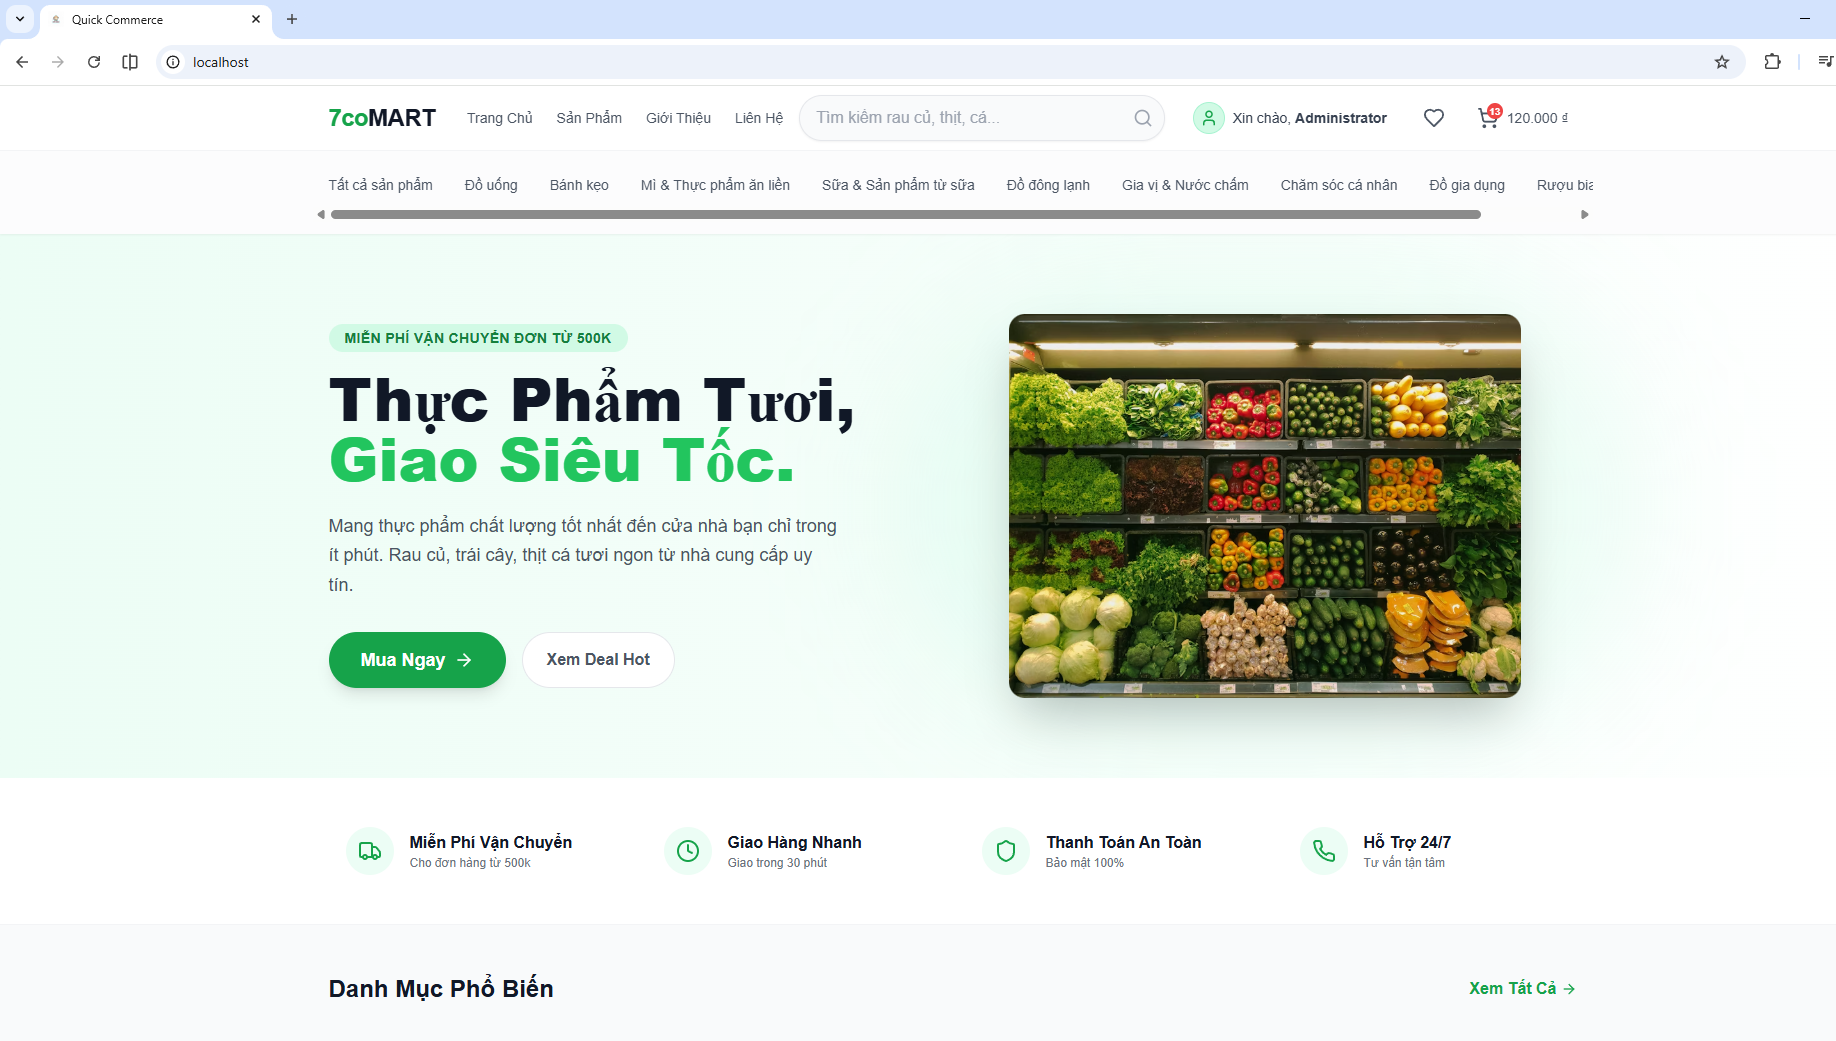
\includegraphics[width=0.85\textwidth]{figs/homepage.png}
    \caption{Giao diện trang chủ mua sắm trực tuyến của hệ thống cửa hàng tiện lợi 7coMART}
    \label{fig:7comart_homepage}
\end{figure}

\textbf{Nhận xét giao diện:} Như được minh họa tại Hình \ref{fig:7comart_homepage}, giao diện trang chủ của 7coMART được thiết kế hiện đại, responsive hoàn toàn. Các khối danh mục sản phẩm tiện lợi được bố trí trực quan giúp người dùng dễ dàng tìm kiếm và lựa chọn sản phẩm nhanh chóng. Ô tìm kiếm nổi bật ở thanh Header là tiêu điểm cho các kịch bản kiểm thử tìm kiếm tiếp theo.

\section{Tổng quan về Kiểm thử phần mềm}

\subsection{Mục tiêu và Tầm quan trọng}
Kiểm thử phần mềm là quá trình khảo sát thực nghiệm một sản phẩm phần mềm nhằm cung cấp cho các bên liên quan thông tin về chất lượng của sản phẩm đó. Đối với 7coMART, kiểm thử phần mềm giúp:
\begin{itemize}
    \item Phát hiện sớm các lỗi logic nghiệp vụ trong việc tính tiền giỏ hàng, trừ kho hàng FEFO trước khi hệ thống chính thức vận hành thương mại.
    \item Đảm bảo an toàn bảo mật, chống các cuộc tấn công đánh cắp tài khoản hoặc can thiệp tham số giá tiền.
    \item Khẳng định hệ thống chạy đúng yêu cầu đặc tả chức năng và đem lại trải nghiệm mua sắm ổn định nhất cho người dùng.
\end{itemize}

\subsection{Áp dụng 7 nguyên tắc kiểm thử phần mềm vào dự án 7coMART}
\begin{enumerate}
    \item \textbf{Kiểm thử chỉ ra sự hiện diện của lỗi (Testing shows presence of defects):} Các kịch bản kiểm thử được thiết kế nhằm tìm kiếm và chứng minh website 7coMART vẫn tồn tại lỗi (như lỗi SQLi, lỗi số lượng âm). Kiểm thử không thể chứng minh hệ thống hoàn hảo 100\% không có lỗi.
    \item \textbf{Kiểm thử toàn diện là bất khả thi (Exhaustive testing is impossible):} Số lượng sản phẩm kết hợp trong giỏ hàng và dữ liệu nhập vào form là vô hạn. Nhóm tập trung thiết kế các kịch bản kiểm thử trọng tâm cho luồng mua sắm chính bằng cách phân lớp dữ liệu.
    \item \textbf{Kiểm thử càng sớm càng tốt (Early testing):} Việc lập kế hoạch và thiết kế kịch bản test được nhóm triển khai ngay sau khi chốt tài liệu đặc tả yêu cầu chức năng, giúp phát hiện lỗi logic ngay trên bản thiết kế trước khi lập trình viên bắt tay viết code.
    \item \textbf{Sự tập trung của lỗi (Defects clustering):} Lỗi thường tập trung nhiều ở những mô-đun phức tạp. Trong 7coMART, lỗi chủ yếu nằm ở mô-đun đặt hàng kết hợp với khóa đồng thời trừ kho PostgreSQL và kiểm soát hạn sử dụng.
    \item \textbf{Nghịch lý thuốc trừ sâu (Pesticide paradox):} Nếu liên tục lặp lại một bộ test cases cũ, nhóm sẽ không tìm thêm được lỗi mới. Vì vậy, bộ kịch bản test luôn được cập nhật, bổ sung các ca kiểm thử biên và giá trị ngẫu nhiên.
    \item \textbf{Kiểm thử phụ thuộc vào ngữ cảnh (Testing is context dependent):} 7coMART is một ứng dụng thương mại điện tử, do đó ngữ cảnh kiểm thử cực kỳ coi trọng tính toàn vẹn dữ liệu giỏ hàng, giao dịch đặt hàng và tính bảo mật của mã hóa mật khẩu.
    \item \textbf{Sự ngộ nhận về việc không có lỗi (Absence-of-errors fallacy):} Một hệ thống 7coMART được test sạch bóng lỗi kỹ thuật vẫn là thất bại nếu giao diện quá khó dùng, luồng đặt hàng rườm rà khiến khách hàng bỏ đi. Nhóm luôn kiểm định dựa trên trải nghiệm khách hàng thực tế.
\end{enumerate}

\subsection{Phân biệt Kiểm thử Chức năng và Kiểm thử Phi chức năng}
\begin{table}[H]
\centering
\caption{So sánh Kiểm thử Chức năng và Phi chức năng tại 7coMART}
\renewcommand{\arraystretch}{1.3}
\begin{tabular}{|p{2.2cm}|p{6cm}|p{6cm}|}
\hline
\textbf{Tiêu chí} & \textbf{Kiểm thử Chức năng} & \textbf{Kiểm thử Phi chức năng} \\ \hline
\textbf{Mục tiêu} & Kiểm tra hệ thống làm ĐÚNG chức năng yêu cầu hay không. & Kiểm tra hệ thống hoạt động TỐT như thế nào (hiệu năng, bảo mật). \\ \hline
\textbf{Đối tượng} & Đăng nhập thành công, tìm thấy sản phẩm, thêm đúng số lượng giỏ hàng, tạo đơn hàng trừ kho đúng lô FEFO. & Thời gian phản hồi API dưới 200ms, mã hóa mật khẩu bằng bcrypt, chống tấn công SQLi, XSS. \\ \hline
\textbf{Công cụ} & Manual test trên trình duyệt, Postman gọi API. & JMeter (tải), OWASP ZAP (bảo mật), Lighthouse. \\ \hline
\end{tabular}
\end{table}

\section{Tổng quan về công cụ quản lý lỗi Mantis Bug Tracker}
Mantis Bug Tracker (MantisBT) là một hệ thống theo dõi lỗi phần mềm mã nguồn mở dựa trên web. Công cụ cung cấp một quy trình chuyên nghiệp giúp Tester ghi nhận lỗi một cách chi tiết và phân công cho Lập trình viên xử lý, theo sát vòng đời lỗi từ lúc phát hiện cho tới khi được khắc phục hoàn toàn. Sự tích hợp Mantis giúp tăng cường tính minh bạch, rút ngắn khoảng cách giao tiếp giữa các thành viên dự án và tự động hóa các đo lường báo cáo chất lượng phần mềm.
\chapter{LẬP KẾ HOẠCH VÀ THIẾT KẾ KỊCH BẢN KIỂM THỬ}

\section{Phạm vi kiểm thử theo từng Sprint}
Nhằm đảm bảo quá trình kiểm thử được triển khai khoa học, nhóm đã phân chia phạm vi kiểm thử thành 02 Sprint thực hành trọng tâm, tập trung vào luồng tương tác cốt lõi của khách hàng:
\begin{itemize}
    \item \textbf{Sprint 1 (Xác thực và Tra cứu sản phẩm):}
    \begin{itemize}
        \item Tính năng Đăng ký tài khoản mới và Đăng nhập hệ thống (Phân quyền Customer/Staff/Admin).
        \item Tính năng Tìm kiếm sản phẩm theo tên và Lọc sản phẩm theo danh mục ngành hàng.
    \end{itemize}
    \item \textbf{Sprint 2 (Giỏ hàng và Quy trình đặt hàng):}
    \begin{itemize}
        \item Các thao tác thêm sản phẩm vào giỏ, điều chỉnh tăng/giảm số lượng sản phẩm, xóa sản phẩm khỏi giỏ hàng.
        \item Luồng xác nhận đơn hàng, ràng buộc số lượng tồn kho thực tế, áp dụng quy tắc FEFO khi xuất kho hàng hóa.
    \end{itemize}
\end{itemize}

\section{Áp dụng các kỹ thuật kiểm thử Hộp đen (Black-box Testing)}
Kiểm thử hộp đen tập trung hoàn toàn vào đầu vào và đầu ra của phần mềm dựa trên tài liệu đặc tả chức năng, không đòi hỏi Tester phải hiểu rõ cấu trúc mã nguồn bên trong Python FastAPI hay React. Nhóm áp dụng 3 kỹ thuật kinh điển để tối ưu hóa bộ kịch bản kiểm thử:

\subsection{Kỹ thuật Phân lớp tương đương (Equivalence Partitioning)}
Kỹ thuật này chia miền đầu vào của chương trình thành các lớp dữ liệu tương đương nhau, đại diện cho hành vi xử lý giống nhau của hệ thống. Ta chỉ cần chọn một giá trị đại diện trong mỗi lớp để kiểm thử, giúp giảm thiểu đáng kể số ca kiểm thử cần chạy.

\noindent\textbf{Áp dụng cho Form Đăng nhập 7coMART:}
\begin{itemize}
    \item \textbf{Trường Email:}
    \begin{itemize}
        \item Lớp hợp lệ ($EC_1$): Địa chỉ email đúng cấu trúc tiêu chuẩn (Ví dụ: \texttt{khach1@gmail.com}).
        \item Lớp không hợp lệ ($EC_2$): Email thiếu ký tự \texttt{@} (Ví dụ: \texttt{khach1gmail.com}).
        \item Lớp không hợp lệ ($EC_3$): Email thiếu tên miền (Ví dụ: \texttt{khach1@.com} hoặc \texttt{khach1@gmail}).
        \item Lớp không hợp lệ ($EC_4$): Email bỏ trống.
    \end{itemize}
    \item \textbf{Trường Mật khẩu:}
    \begin{itemize}
        \item Lớp hợp lệ ($EC_5$): Mật khẩu có độ dài từ 8 đến 20 ký tự (Ví dụ: \texttt{password123}).
        \item Lớp không hợp lệ ($EC_6$): Mật khẩu quá ngắn dưới 8 ký tự (Ví dụ: \texttt{pass12}).
        \item Lớp không hợp lệ ($EC_7$): Mật khẩu quá dài trên 20 ký tự.
        \item Lớp không hợp lệ ($EC_8$): Mật khẩu để trống.
    \end{itemize}
\end{itemize}

\subsection{Kỹ thuật Phân tích giá trị biên (Boundary Value Analysis)}
Lỗi phần mềm thường tập trung rất cao ở ranh giới của các miền giá trị đầu vào thay vì ở giữa. Kỹ thuật này lựa chọn các giá trị tại biên và các giá trị ngay sát biên để thực thi kiểm thử.

\noindent\textbf{Áp dụng cho số lượng sản phẩm thêm vào giỏ hàng (Quantity):}
Giả sử số lượng tồn kho thực tế của mặt hàng sữa tươi TH True Milk trong hệ thống tại lô hàng hiện tại là $N = 50$ hộp. Số lượng đặt hàng hợp lệ phải nằm trong khoảng $[1, 50]$. Các giá trị biên được xác định gồm:
\begin{itemize}
    \item Biên dưới hợp lệ tối thiểu: $1$ (Hệ thống chấp nhận thêm thành công).
    \item Giá trị sát dưới không hợp lệ: $0$ (Hệ thống từ chối, hiển thị thông báo lỗi số lượng tối thiểu phải bằng 1).
    \item Giá trị cực biên âm: $-1$ (Hệ thống ngăn chặn, không cho phép nhập số lượng âm).
    \item Biên trên hợp lệ tối đa: $50$ (Hệ thống chấp nhận, lấy toàn bộ tồn kho của lô hiện tại).
    \item Giá trị vượt sát biên trên: $51$ (Hệ thống từ chối, thông báo không đủ số lượng hàng tồn kho cung cấp).
    \item Giá trị vượt xa biên trên: $100$ (Hệ thống từ chối, cảnh báo vượt quá giới hạn kho).
\end{itemize}

\subsection{Kỹ thuật Bảng quyết định (Decision Table)}
Kỹ thuật bảng quyết định được sử dụng để thiết kế kịch bản test cho các tính năng chứa logic nghiệp vụ phức tạp, chịu sự chi phối đồng thời của nhiều điều kiện đầu vào khác nhau.

\noindent\textbf{Áp dụng cho logic áp dụng mã giảm giá thanh toán (Discount Coupon):}
\begin{itemize}
    \item \textbf{Các điều kiện đầu vào (Conditions):}
    \begin{enumerate}
        \item $C_1$: Nhập đúng mã giảm giá đang hoạt động (Ví dụ: \texttt{COOP10}). (True/False)
        \item $C_2$: Tổng giá trị đơn hàng đạt điều kiện tối thiểu $\ge 100.000$ VNĐ. (True/False)
        \item $C_3$: Mã giảm giá còn lượt sử dụng và còn thời hạn hiệu lực. (True/False)
    \end{enumerate}
    \item \textbf{Các hành động tương ứng (Actions):}
    \begin{enumerate}
        \item $A_1$: Áp dụng mã giảm giá thành công, giảm trừ trực tiếp 10\% vào tổng hóa đơn.
        \item $A_2$: Hiển thị cảnh báo lỗi tương ứng với điều kiện bị vi phạm.
    \end{enumerate}
\end{itemize}

\begin{table}[H]
\centering
\caption{Bảng quyết định logic áp dụng mã giảm giá tại 7coMART}
\renewcommand{\arraystretch}{1.2}
\begin{tabular}{|l|c|c|c|c|c|c|c|c|}
\hline
\textbf{Điều kiện / Luật} & \textbf{R1} & \textbf{R2} & \textbf{R3} & \textbf{R4} & \textbf{R5} & \textbf{R6} & \textbf{R7} & \textbf{R8} \\ \hline
$C_1$: Mã giảm giá hợp lệ? & Y & Y & Y & Y & N & N & N & N \\ \hline
$C_2$: Giá trị đơn hàng $\ge 100k$? & Y & Y & N & N & Y & Y & N & N \\ \hline
$C_3$: Mã còn lượt/còn hạn? & Y & N & Y & N & Y & N & Y & N \\ \hline
\hline
$A_1$: Áp dụng thành công (Giảm 10\%) & \cellcolor{green!20}\textbf{X} & & & & & & & \\ \hline
$A_2$: Hiển thị thông báo lỗi & & \cellcolor{red!20}\textbf{X} & \cellcolor{red!20}\textbf{X} & \cellcolor{red!20}\textbf{X} & \cellcolor{red!20}\textbf{X} & \cellcolor{red!20}\textbf{X} & \cellcolor{red!20}\textbf{X} & \cellcolor{red!20}\textbf{X} \\ \hline
\end{tabular}
\end{table}

\section{Danh sách Kịch bản kiểm thử (Test Cases) chi tiết}
Dưới đây là tập hợp 15 kịch bản kiểm thử cốt lõi được thiết kế chi tiết bằng bảng LaTeX, bao phủ toàn bộ phạm vi kiểm thử đã vạch ra của Sprint 1 và Sprint 2 trên hệ thống cửa hàng tiện lợi 7coMART.

\begin{table}[H]
\centering
\caption{Kịch bản kiểm thử chi tiết - Sprint 1 (Xác thực \& Tìm kiếm)}
\renewcommand{\arraystretch}{1.2}
\small
\begin{tabular}{|p{1.2cm}|p{1.8cm}|p{3.5cm}|p{2.5cm}|p{5.5cm}|}
\hline
\textbf{Mã TC} & \textbf{Mô-đun} & \textbf{Mục tiêu kiểm thử} & \textbf{Dữ liệu vào} & \textbf{Kết quả mong đợi} \\ \hline
\texttt{TC\_01} & Đăng ký & Kiểm tra đăng ký thành công với thông tin hợp lệ. & Email, mật khẩu, tên hợp lệ. & Đăng ký thành công, thông báo kích hoạt tài khoản và chuyển hướng tới Login. \\ \hline
\texttt{TC\_02} & Đăng ký & Kiểm tra đăng ký thất bại khi Email sai định dạng. & Email thiếu \texttt{@} (\texttt{testgmail.com}) & Hiển thị thông báo lỗi email không đúng định dạng chuẩn. \\ \hline
\texttt{TC\_03} & Đăng ký & Kiểm tra đăng ký thất bại khi mật khẩu quá ngắn. & Mật khẩu 6 ký tự (\texttt{123456}) & Hiển thị cảnh báo lỗi độ dài mật khẩu tối thiểu phải từ 8 ký tự trở lên. \\ \hline
\texttt{TC\_04} & Đăng ký & Kiểm tra đăng ký thất bại khi email đã tồn tại. & Email trùng lặp hệ thống. & Thông báo lỗi email đã được đăng ký sử dụng trước đó. \\ \hline
\texttt{TC\_05} & Đăng nhập & Kiểm tra đăng nhập thành công với vai trò Khách hàng. & \texttt{khach1@gmail.com} mật khẩu đúng. & Đăng nhập thành công, lưu JWT Token và chuyển hướng về trang chủ mua sắm. \\ \hline
\texttt{TC\_06} & Đăng nhập & Kiểm tra đăng nhập thất bại khi sai mật khẩu. & Email đúng, mật khẩu sai. & Hiển thị thông báo lỗi tài khoản hoặc mật khẩu không chính xác. \\ \hline
\texttt{TC\_07} & Tìm kiếm & Tìm kiếm thành công sản phẩm với từ khóa tiếng Việt. & Từ khóa: ``sữa tươi'' & Hiển thị danh sách các sản phẩm sữa tươi TH, Vinamilk tương ứng. \\ \hline
\texttt{TC\_08} & Tìm kiếm & Kiểm tra tìm kiếm không tìm thấy sản phẩm. & Từ khóa: ``linh kiện pc'' & Hiển thị thông báo không tìm thấy sản phẩm phù hợp. \\ \hline
\end{tabular}
\end{table}

\begin{table}[H]
\centering
\caption{Kịch bản kiểm thử chi tiết - Sprint 2 (Giỏ hàng \& Đặt hàng)}
\renewcommand{\arraystretch}{1.2}
\small
\begin{tabular}{|p{1.2cm}|p{1.8cm}|p{3.5cm}|p{2.5cm}|p{5.5cm}|}
\hline
\textbf{Mã TC} & \textbf{Mô-đun} & \textbf{Mục tiêu kiểm thử} & \textbf{Dữ liệu vào} & \textbf{Kết quả mong đợi} \\ \hline
\texttt{TC\_09} & Giỏ hàng & Thêm sản phẩm thành công vào giỏ hàng trống. & Click chọn SP sữa tươi, số lượng = 1. & Sản phẩm xuất hiện trong giỏ hàng, tổng tiền cập nhật chính xác. \\ \hline
\texttt{TC\_10} & Giỏ hàng & Kiểm tra thêm số lượng biên bằng $0$ vào giỏ hàng. & Nhập số lượng = 0. & Hệ thống báo lỗi số lượng không hợp lệ (phải $\ge 1$). \\ \hline
\texttt{TC\_11} & Giỏ hàng & Kiểm tra chặn thêm số lượng âm vào giỏ hàng. & Nhập số lượng = -5. & Không cho phép nhập âm, tự động reset về 1 hoặc báo lỗi tham số. \\ \hline
\texttt{TC\_12} & Giỏ hàng & Kiểm tra thêm vượt số lượng tồn kho tối đa. & Nhập số lượng lớn hơn tồn kho thực tế. & Thông báo không đủ số lượng hàng tồn kho cung cấp. \\ \hline
\texttt{TC\_13} & Đặt hàng & Đặt hàng thành công với giỏ hàng hợp lệ. & Click thanh toán, chọn COD. & Tạo đơn hàng thành công, trừ kho đúng lô hàng hết hạn trước (FEFO). \\ \hline
\texttt{TC\_14} & Đặt hàng & Áp dụng thành công mã giảm giá hợp lệ. & Nhập mã \texttt{COOP10} đơn hàng $\ge 100k$. & Đơn hàng được giảm trực tiếp 10\% tổng giá trị hóa đơn thanh toán. \\ \hline
\texttt{TC\_15} & Đặt hàng & Áp dụng thất bại mã giảm giá khi đơn hàng dưới 100k. & Nhập mã \texttt{COOP10} đơn hàng $50k$. & Báo lỗi đơn hàng chưa đạt giá trị tối thiểu để sử dụng mã ưu đãi. \\ \hline
\end{tabular}
\end{table}
\chapter{THỰC THI KIỂM THỬ VÀ QUẢN LÝ LỖI TRÊN MANTIS}

\section{Thiết lập môi trường và Thực thi kiểm thử}

\subsection{Môi trường thực thi kiểm thử}
Quá trình kiểm thử website cửa hàng tiện lợi 7coMART được thực thi trên môi trường máy chủ cục bộ đồng bộ hóa bằng Docker Compose với các cấu hình phần mềm cụ thể sau:
\begin{itemize}
    \item \textbf{Địa chỉ ứng dụng:} \url{http://localhost} (Cổng HTTP chuẩn được phục vụ bởi Nginx Reverse Proxy).
    \item \textbf{Địa chỉ API Backend:} \url{http://localhost:8000/docs} (Swagger UI phục vụ gọi test API độc lập).
    \item \textbf{Hệ điều hành kiểm thử:} Microsoft Windows 11 Enterprise.
    \item \textbf{Trình duyệt sử dụng:} Google Chrome (Version 122 ổn định) kết hợp công cụ Chrome Developer Tools (F12) để theo dõi luồng mạng Network Tab và ghi nhận lỗi JavaScript Console.
\end{itemize}

\subsection{Quy trình và Quy ước ghi nhận kết quả thực thi}
Tester tiến hành duyệt qua từng kịch bản kiểm thử đã định nghĩa ở Chương 2, thao tác trực tiếp trên giao diện người dùng và tiến hành đối chiếu Kết quả thực tế (\textit{Actual Result}) với Kết quả mong đợi (\textit{Expected Result}). Trạng thái của kịch bản test được đánh giá theo quy ước:
\begin{itemize}
    \item \textbf{Đạt (Pass - P):} Khi hệ thống phản hồi chính xác, Kết quả thực tế trùng khớp hoàn toàn với Kết quả mong đợi.
    \item \textbf{Lỗi (Fail - F):} Khi hệ thống phản hồi sai logic nghiệp vụ, phát sinh lỗi Crash trang, lỗi 500 API hoặc xuất hiện lỗ hổng bảo mật nghiêm trọng. Mọi ca kiểm thử mang trạng thái Fail đều bắt buộc phải được lập báo cáo lỗi (Defect Report) và đẩy lên hệ thống quản lý lỗi trực tuyến Mantis Bug Tracker.
\end{itemize}

\subsection{Minh họa giao diện thực thi kiểm thử các Sprints}
Dưới đây là một số hình ảnh chụp màn hình ghi nhận giao diện thực tế của website 7coMART trong quá trình nhóm tiến hành thực thi kiểm thử thủ công cho Sprint 1 và Sprint 2:

\begin{figure}[H]
    \centering
    \begin{minipage}{0.48\textwidth}
        \centering
        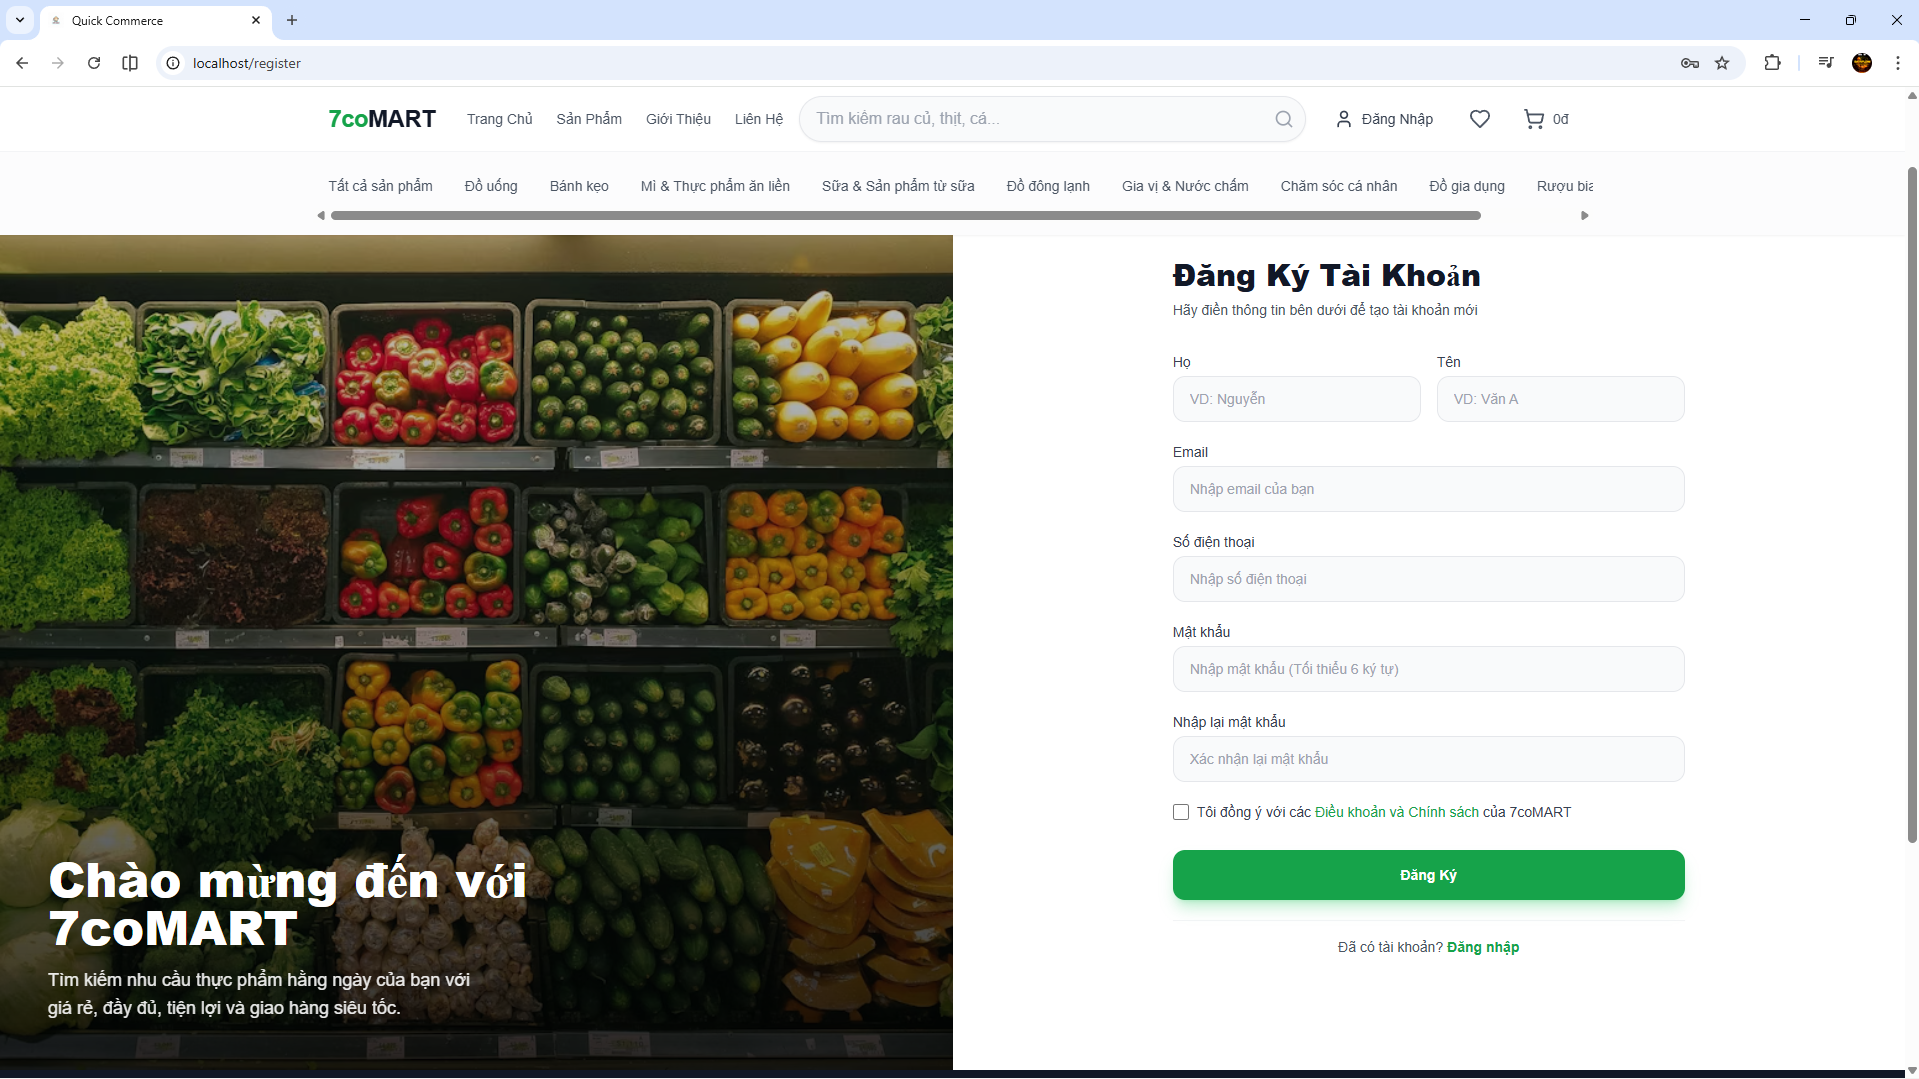
\includegraphics[width=\textwidth]{figs/register.png}
        \caption{Giao diện form Đăng ký tài khoản mới của hệ thống 7coMART}
        \label{fig:register_ui}
    \end{minipage}
    \hfill
    \begin{minipage}{0.48\textwidth}
        \centering
        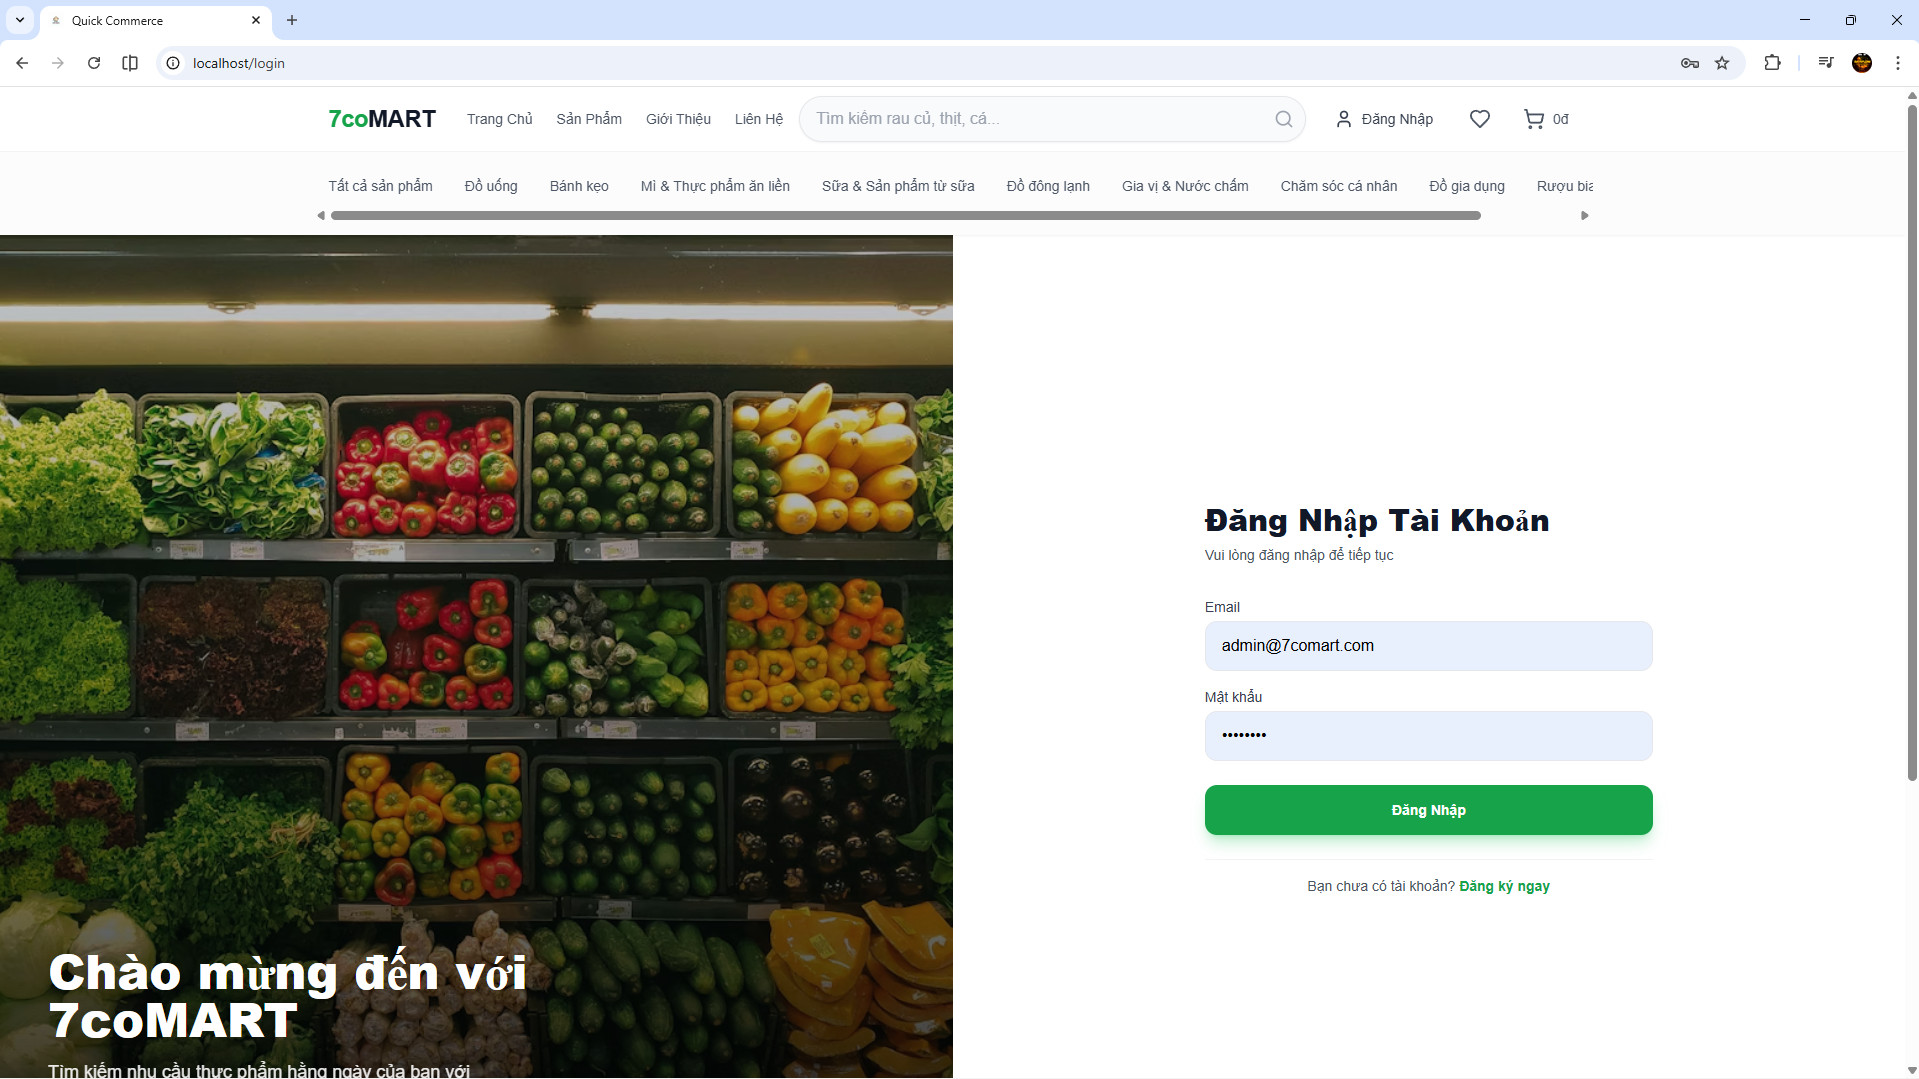
\includegraphics[width=\textwidth]{figs/login.png}
        \caption{Giao diện form Đăng nhập tài khoản của hệ thống 7coMART}
        \label{fig:login_ui}
    \end{minipage}
\end{figure}

Hình \ref{fig:register_ui} và \ref{fig:login_ui} thể hiện sự hoạt động bình thường, đúng nghiệp vụ của các chức năng Xác thực của Khách hàng trong Sprint 1 trước khi tiến hành các kịch bản kiểm tra lỗi.

\begin{figure}[H]
    \centering
    \begin{minipage}{0.48\textwidth}
        \centering
        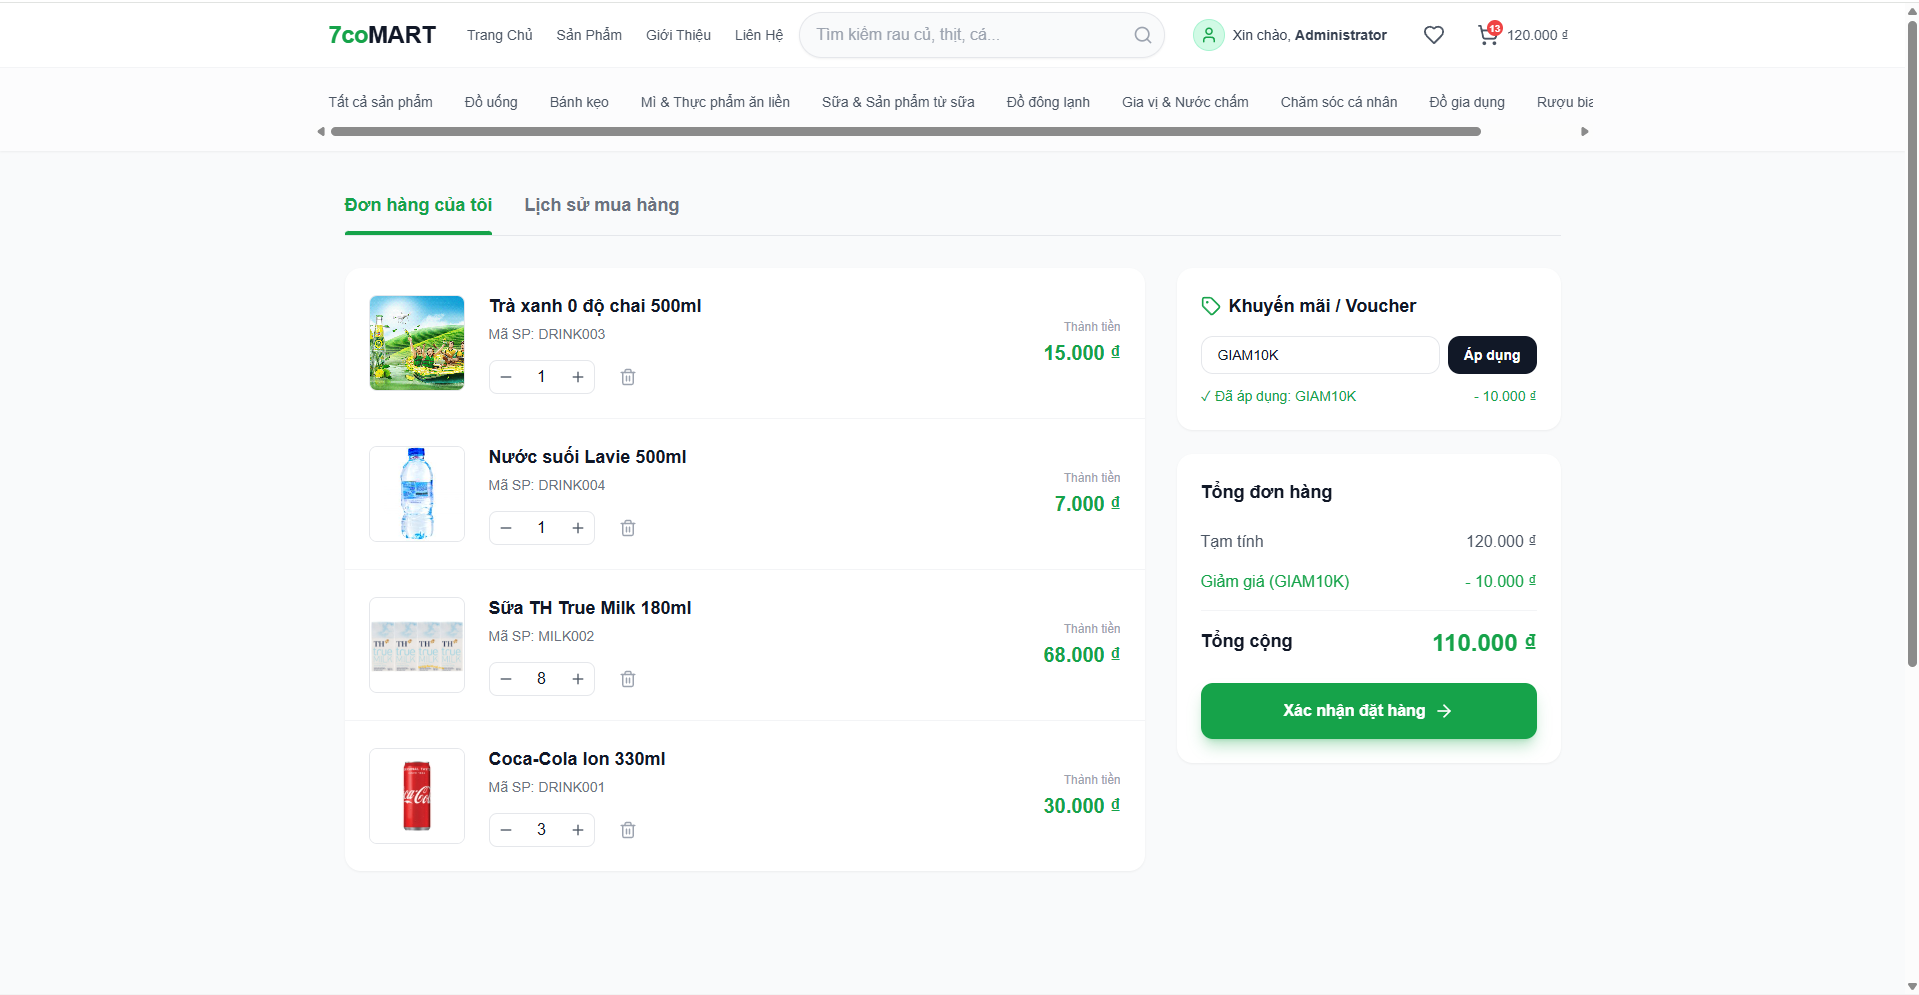
\includegraphics[width=\textwidth]{figs/cart.png}
        \caption{Giao diện Giỏ hàng với các sản phẩm được chọn trong Sprint 2}
        \label{fig:cart_ui}
    \end{minipage}
    \hfill
    \begin{minipage}{0.48\textwidth}
        \centering
        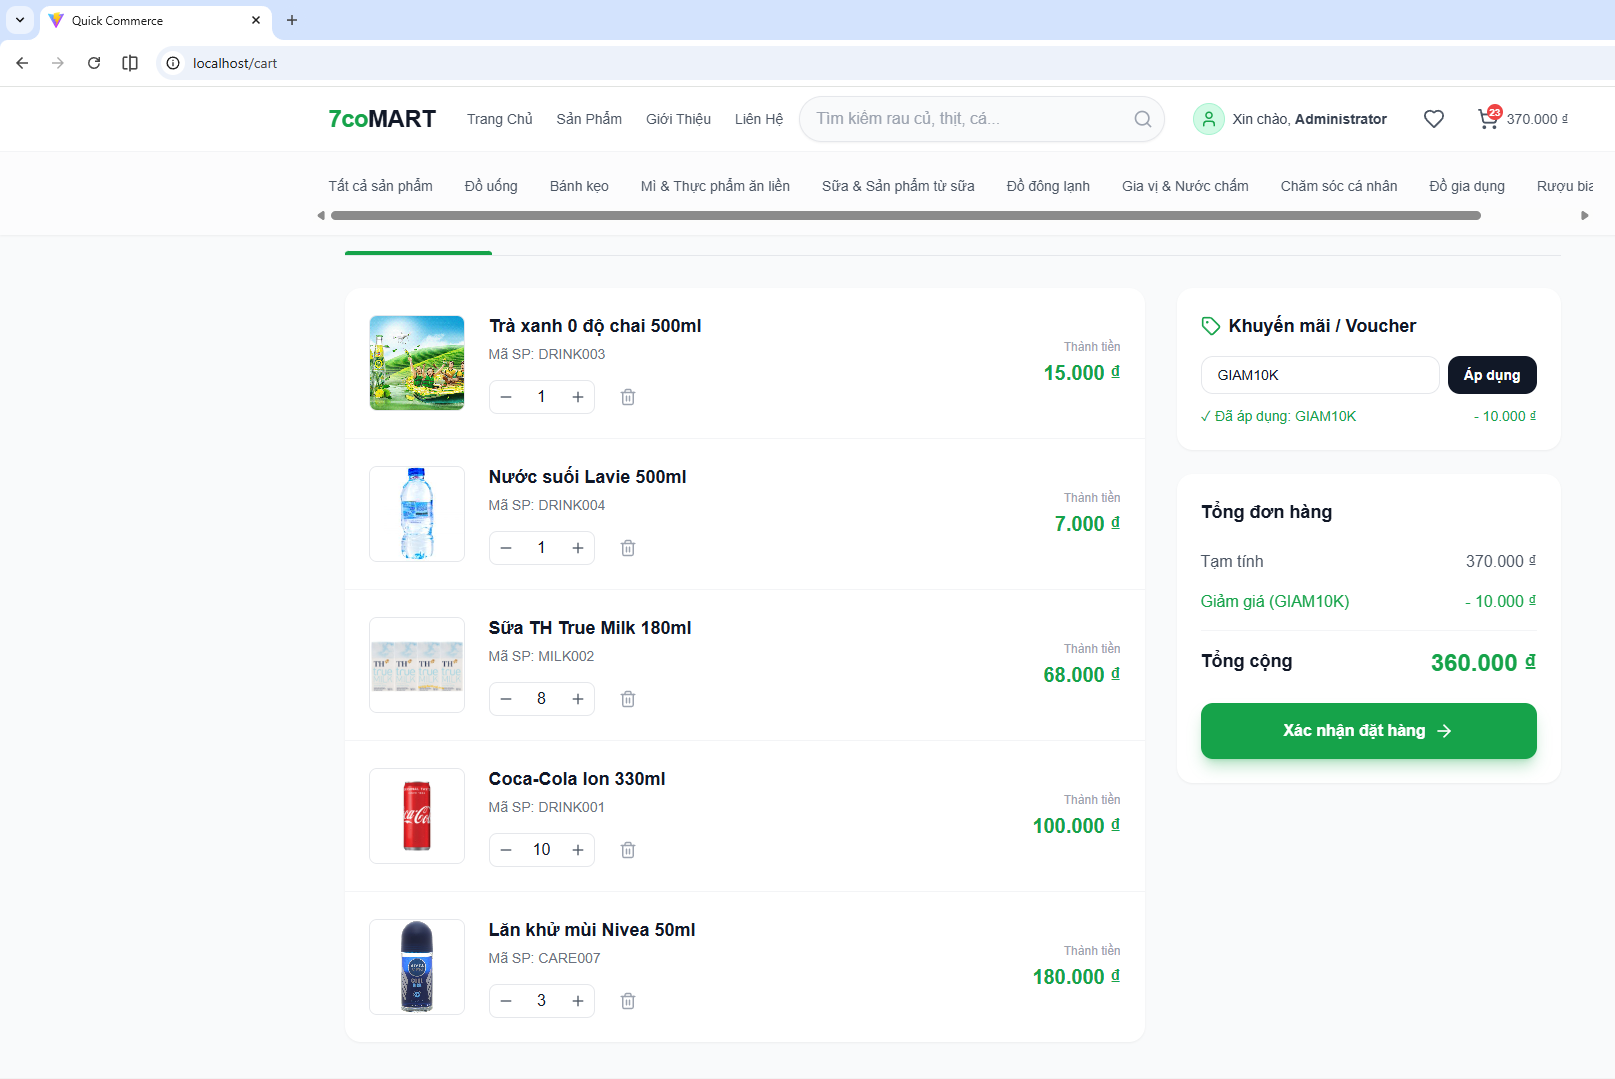
\includegraphics[width=\textwidth]{figs/test_cart_result.png}
        \caption{Giao diện thanh toán và kiểm định logic giỏ hàng}
        \label{fig:cart_result_ui}
    \end{minipage}
\end{figure}

Như được minh họa tại Hình \ref{fig:cart_ui} và \ref{fig:cart_result_ui}, hệ thống giỏ hàng của 7coMART hiển thị chính xác tên sản phẩm, đơn giá, tổng giá tiền tạm tính thời gian thực và cho phép cập nhật số lượng trơn tru đối với các ca kiểm thử hợp lệ.

\section{Quản lý vòng đời lỗi chuyên nghiệp với Mantis Bug Tracker}

\subsection{Sơ đồ vòng đời lỗi trong LaTeX bằng TikZ}
Để duy trì quy trình sửa lỗi nhất quán, nhóm áp dụng sơ đồ chuyển đổi trạng thái lỗi chuẩn của MantisBT. Dưới đây là sơ đồ vòng đời lỗi được vẽ trực tiếp bằng thư viện TikZ sắc nét:

\begin{center}
\begin{tikzpicture}[node distance=2.5cm, auto]
    % Define styles
    \tikzstyle{state} = [rectangle, rounded corners, minimum width=2.5cm, minimum height=1cm, text centered, draw=blue!80, fill=blue!10, thick]
    \tikzstyle{line} = [draw, -latex, thick, blue!80]
    
    % Place nodes
    \node [state] (new) {NEW (Tester phát hiện)};
    \node [state, right of=new, node distance=4.5cm] (assigned) {ASSIGNED (Dev nhận lỗi)};
    \node [state, right of=assigned, node distance=4.5cm] (resolved) {RESOLVED (Đã vá lỗi)};
    \node [state, below of=resolved, node distance=2.5cm] (closed) {CLOSED (Tester đóng lỗi)};
    
    % Draw edges
    \path [line] (new) -- (assigned);
    \path [line] (assigned) -- (resolved);
    \path [line] (resolved) -- (closed);
    \path [line] (resolved) |- node [near end, above] {Re-test Fail} (new);
\end{tikzpicture}
\end{center}

\subsection{Quy trình viết Báo cáo lỗi (Defect Report) chuẩn chỉnh}
Một Báo cáo lỗi chuyên nghiệp trên Mantis bắt buộc phải cung cấp đầy đủ thông tin để Lập trình viên có thể dễ dàng tái hiện lỗi và tiến hành sửa đổi mã nguồn:
\begin{enumerate}
    \item \textbf{Summary (Tiêu đề):} Mô tả cực kỳ ngắn gọn, định danh vị trí lỗi (Ví dụ: \texttt{[Cart API] Lỗi nhập số lượng âm rút tiền hệ thống}).
    \item \textbf{Description (Mô tả chi tiết):} Nêu rõ hành vi không mong muốn của hệ thống và ảnh hưởng của nó.
    \item \textbf{Steps to Reproduce (Các bước tái hiện):} Liệt kê các bước thao tác tuần tự (1, 2, 3...) để bất kỳ ai cũng có thể kích hoạt lại đúng lỗi đó trên máy của mình.
    \item \textbf{Severity (Mức độ nghiêm trọng):} Phân cấp mức độ ảnh hưởng (Block, Crash, Major, Minor).
    \item \textbf{Priority (Độ ưu tiên):} Đánh giá mức độ khẩn cấp cần sửa (Urgent, High, Normal, Low).
\end{enumerate}

\begin{figure}[H]
    \centering
    \begin{tikzpicture}[scale=0.8, every node/.style={transform shape}]
        % Browser border
        \draw[thick, fill=white] (0,0) rectangle (15,9.5);
        % Browser title bar
        \draw[fill=gray!20, thick] (0,8.7) rectangle (15,9.5);
        % Red, yellow, green window controls
        \fill[red] (0.3,9.15) circle (0.12);
        \fill[yellow] (0.7,9.15) circle (0.12);
        \fill[green] (1.1,9.15) circle (0.12);
        % Address bar
        \draw[fill=white, rounded corners=2pt] (2.0,8.85) rectangle (12.0,9.35);
        \node[right] at (2.2,9.1) {\scriptsize \texttt{http://localhost:8089/view\_all\_bug\_page.php}};
        
        % Left Sidebar (MantisBT menu)
        \draw[fill=gray!80, draw=none] (0,0) rectangle (2.5,8.7);
        \node[white, right] at (0.2,8.3) {\small\textbf{MantisBT v2.25}};
        \draw[white!50] (0.2,8.0) -- (2.3,8.0);
        \node[white, right] at (0.3,7.5) {\tiny $\bullet$ Bảng điều khiển};
        \node[white, right] at (0.3,7.0) {\tiny $\bullet$ Xem danh sách lỗi};
        \node[white, right] at (0.3,6.5) {\tiny $\bullet$ Báo cáo lỗi};
        \node[white, right] at (0.3,6.0) {\tiny $\bullet$ Quản lý hệ thống};
        
        % Main Workspace Header
        \node[right] at (2.8,8.2) {\small\textbf{Danh sách sự cố lỗi đã ghi nhận (7coMART)}};
        \draw[gray!30] (2.8,7.8) -- (14.5,7.8);
        
        % Table Header
        \draw[fill=gray!20, draw=gray] (2.8,7.0) rectangle (14.5,7.5);
        \node[right] at (2.9,7.25) {\tiny\textbf{ID}};
        \node[right] at (3.8,7.25) {\tiny\textbf{Danh mục}};
        \node[right] at (5.8,7.25) {\tiny\textbf{Mức độ}};
        \node[right] at (7.2,7.25) {\tiny\textbf{Trạng thái}};
        \node[right] at (8.8,7.25) {\tiny\textbf{Tóm tắt sự cố}};
        
        % Row 1: SQL Injection
        \draw[draw=gray] (2.8,6.2) rectangle (14.5,7.0);
        \node[right] at (2.9,6.6) {\tiny \texttt{0000021}};
        \node[right] at (3.8,6.6) {\tiny Xác thực (Auth)};
        \node[right, fill=red!20, rounded corners=2.5pt] at (5.8,6.6) {\tiny\textbf{Block}};
        \node[right, fill=orange!20, rounded corners=2.5pt] at (7.2,6.6) {\tiny\textbf{New}};
        \node[right] at (8.8,6.6) {\tiny [Login] Lỗ hổng bảo mật SQL Injection tại form Đăng nhập};
        
        % Row 2: Unicode Search
        \draw[draw=gray] (2.8,5.4) rectangle (14.5,6.2);
        \node[right] at (2.9,5.8) {\tiny \texttt{0000022}};
        \node[right] at (3.8,5.8) {\tiny Tìm kiếm (Catalog)};
        \node[right, fill=orange!10, rounded corners=2.5pt] at (5.8,5.8) {\tiny\textbf{Major}};
        \node[right, fill=blue!20, rounded corners=2.5pt] at (7.2,5.8) {\tiny\textbf{Assigned}};
        \node[right] at (8.8,5.8) {\tiny Lỗi 500 Internal Server Error khi tìm tiếng Việt Unicode};
        
        % Row 3: Negative quantity
        \draw[draw=gray] (2.8,4.6) rectangle (14.5,5.4);
        \node[right] at (2.9,5.0) {\tiny \texttt{0000023}};
        \node[right] at (3.8,5.0) {\tiny Giỏ hàng (Cart)};
        \node[right, fill=red!10, rounded corners=2.5pt] at (5.8,5.0) {\tiny\textbf{Critical}};
        \node[right, fill=green!20, rounded corners=2.5pt] at (7.2,5.0) {\tiny\textbf{Resolved}};
        \node[right] at (8.8,5.0) {\tiny Hacker can thiệp sửa đổi số lượng âm giỏ hàng qua HTTP};
        
        % Row 4: Interface small bug
        \draw[draw=gray] (2.8,3.8) rectangle (14.5,4.6);
        \node[right] at (2.9,4.2) {\tiny \texttt{0000024}};
        \node[right] at (3.8,4.2) {\tiny Giao diện (UI)};
        \node[right, fill=gray!20, rounded corners=2.5pt] at (5.8,4.2) {\tiny\textbf{Minor}};
        \node[right, fill=green!20, rounded corners=2.5pt] at (7.2,4.2) {\tiny\textbf{Closed}};
        \node[right] at (8.8,4.2) {\tiny Lỗi tràn viền nút bấm mua sản phẩm nhanh trên mobile};
    \end{tikzpicture}
    \caption{Giao diện bảng điều khiển quản lý và theo dõi lỗi Mantis Bug Tracker của dự án 7coMART}
    \label{fig:mantis_dashboard}
\end{figure}

\textbf{Nhận xét Hệ thống:} Qua giao diện Dashboard tại Hình \ref{fig:mantis_dashboard}, các lỗi được lập chỉ mục khoa học với màu sắc nhận diện trạng thái trực quan, giúp ban quản trị dự án nhanh chóng đánh giá số lượng lỗi tồn đọng và phân phối nhiệm vụ vá lỗi hiệu quả cho các Lập trình viên.

\section{Thống kê và Chi tiết một số lỗi (Bugs) tiêu biểu}
Dưới đây là chi tiết 03 lỗi nghiêm trọng thực tế được Tester phát hiện trên hệ thống 7coMART và ghi nhận chuẩn xác lên hệ thống ticket Mantis Bug Tracker.

\subsection{Bug 1: Lỗ hổng bảo mật SQL Injection tại Form Đăng nhập}
\begin{itemize}
    \item \textbf{Mã Ticket Mantis:} \texttt{\#0000021}
    \item \textbf{Mô-đun ảnh hưởng:} Xác thực (Authentication / Login API)
    \item \textbf{Mức độ nghiêm trọng:} \textbf{Block (Phong tỏa hệ thống)} - Cho phép vượt qua cơ chế bảo mật đăng nhập.
    \item \textbf{Các bước tái hiện:}
    \begin{enumerate}
        \item Truy cập giao diện Đăng nhập tại địa chỉ \url{http://localhost/login}.
        \item Tại ô email nhập chuỗi ký tự tấn công: \texttt{' OR 1=1 --}
        \item Tại ô mật khẩu nhập giá trị bất kỳ: \texttt{xyz123}
        \item Bấm nút ``Đăng nhập''.
    \end{enumerate}
    \item \textbf{Kết quả thực tế:} Hệ thống bỏ qua bước kiểm tra mật khẩu, tự động đăng nhập thẳng vào tài khoản Quản trị viên (Admin) cấp cao nhất do backend thực thi nối chuỗi SQL thô trực tiếp không qua tham số hóa.
    \item \textbf{Kết quả mong đợi:} Hệ thống phát hiện dữ liệu nhập vào không hợp lệ, từ chối đăng nhập và đưa ra cảnh báo lỗi bảo mật hoặc tài khoản sai.
\end{itemize}

\begin{figure}[H]
    \centering
    \begin{tikzpicture}[scale=0.8, every node/.style={transform shape}]
        % Browser frame
        \draw[thick, fill=white] (0,0) rectangle (15,9.5);
        \draw[fill=gray!20, thick] (0,8.7) rectangle (15,9.5);
        \fill[red] (0.3,9.1) circle (0.12);
        \fill[yellow] (0.7,9.1) circle (0.12);
        \fill[green] (1.1,9.1) circle (0.12);
        \draw[fill=white, rounded corners=2pt] (2.0,8.85) rectangle (12.0,9.35);
        \node[right] at (2.2,9.1) {\scriptsize \texttt{http://localhost:8089/view.php?id=21}};
        
        % Left Sidebar (MantisBT menu)
        \draw[fill=gray!80, draw=none] (0,0) rectangle (2.5,8.7);
        \node[white, right] at (0.3,8.0) {\tiny $\bullet$ Xem danh sách lỗi};
        \node[white, right] at (0.3,7.5) {\tiny $\bullet$ Báo cáo sự cố};
        
        % Main Workspace Header
        \node[right] at (2.8,8.2) {\small\textbf{Xem chi tiết sự cố: \#0000021}};
        \draw[gray!30] (2.8,7.9) -- (14.5,7.9);
        
        % Ticket Details Grid
        \draw[draw=gray, fill=gray!5] (2.8,4.0) rectangle (14.5,7.6);
        % Headers
        \node[right] at (2.9,7.3) {\tiny\textbf{ID:}}; 
        \node[right] at (5.2,7.3) {\tiny 0000021};
        \node[right] at (8.0,7.3) {\tiny\textbf{Danh mục:}}; 
        \node[right] at (10.2,7.3) {\tiny Xác thực (Auth)};
        \draw[gray!20] (2.8,7.0) -- (14.5,7.0);
        
        \node[right] at (2.9,6.7) {\tiny\textbf{Mức độ nghiêm trọng:}}; 
        \node[right, fill=red!20, rounded corners=2pt] at (5.2,6.7) {\tiny\textbf{Block}};
        \node[right] at (8.0,6.7) {\tiny\textbf{Độ ưu tiên:}}; 
        \node[right] at (10.2,6.7) {\tiny Khẩn cấp (Urgent)};
        \draw[gray!20] (2.8,6.4) -- (14.5,6.4);
        
        \node[right] at (2.9,6.1) {\tiny\textbf{Người báo cáo:}}; 
        \node[right] at (5.2,6.1) {\tiny Đinh Minh Đức (Reporter)};
        \node[right] at (8.0,6.1) {\tiny\textbf{Trạng thái:}}; 
        \node[right, fill=orange!20, rounded corners=2pt] at (10.2,6.1) {\tiny\textbf{New}};
        \draw[gray!20] (2.8,5.8) -- (14.5,5.8);
        
        \node[right] at (2.9,5.5) {\tiny\textbf{Tóm tắt:}}; 
        \node[right] at (4.5,5.5) {\tiny\textbf{[Login API] Lỗ hổng SQL Injection tại Form đăng nhập}};
        \draw[gray!20] (2.8,5.2) -- (14.5,5.2);
        
        \node[right] at (2.9,4.7) {\tiny\textbf{Mô tả:}};
        \node[right] at (4.5,4.8) {\tiny Nhập chuỗi độc hại \texttt{' OR 1=1 --} vào ô email cho phép vượt qua};
        \node[right] at (4.5,4.4) {\tiny kiểm định bảo mật mật khẩu và chiếm quyền quản trị Admin.};
        
        % Steps to reproduce
        \draw[draw=gray] (2.8,1.0) rectangle (14.5,3.6);
        \node[right] at (2.9,3.2) {\tiny\textbf{Các bước tái hiện:}};
        \node[right] at (3.1,2.8) {\tiny 1. Truy cập \url{http://localhost/login}};
        \node[right] at (3.1,2.4) {\tiny 2. Nhập email: \texttt{' OR 1=1 --}};
        \node[right] at (3.1,2.0) {\tiny 3. Nhập mật khẩu tùy ý: \texttt{xyz}};
        \node[right] at (3.1,1.6) {\tiny 4. Bấm đăng nhập $\rightarrow$ Đăng nhập thành công và chuyển hướng về tài khoản Admin.};
    \end{tikzpicture}
    \caption{Chi tiết ticket lỗi bảo mật SQL Injection trên form Đăng nhập được ghi nhận trên MantisBT}
    \label{fig:bug_sqli}
\end{figure}

\textbf{Phân tích rủi ro:} Lỗi được chỉ ra tại Hình \ref{fig:bug_sqli} là lỗ hổng bảo mật cực kỳ nguy hại. Một kẻ tấn công ngoài mạng có thể dễ dàng kiểm soát toàn bộ cơ sở dữ liệu khách hàng, sửa đổi giá tiền sản phẩm hoặc chiếm quyền quản trị tối cao của 7coMART mà không cần bất cứ kiến thức mật khẩu nào.

\subsection{Bug 2: Lỗi 500 Internal Server Error khi tìm kiếm từ khóa tiếng Việt chứa Unicode}
\begin{itemize}
    \item \textbf{Mã Ticket Mantis:} \texttt{\#0000022}
    \item \textbf{Mô-đun ảnh hưởng:} Tra cứu sản phẩm (Catalog Search API)
    \item \textbf{Mức độ nghiêm trọng:} \textbf{Major (Lỗi lớn)} - Làm tê liệt chức năng tìm kiếm sản phẩm của người dùng Việt.
    \item \textbf{Các bước tái hiện:}
    \begin{enumerate}
        \item Truy cập trang chủ bán hàng \url{http://localhost}.
        \item Gõ từ khóa tìm kiếm có dấu: ``sữa tươi'' hoặc ``mì ăn liền'' vào ô tìm kiếm.
        \item Nhấn phím Enter hoặc nút Tìm kiếm.
    \end{enumerate}
    \item \textbf{Kết quả thực tế:} Giao diện quay vô tận, Console báo lỗi mạng, gọi API trả về mã lỗi \texttt{500 Internal Server Error} từ backend FastAPI do cơ sở dữ liệu gặp sự cố đối chiếu bảng mã Unicode của PostgreSQL.
    \item \textbf{Kết quả mong đợi:} Hệ thống hiển thị danh sách các sản phẩm sữa tươi hoặc mì gói bình thường, xử lý trơn tru bảng mã tiếng Việt UTF-8.
\end{itemize}

\begin{figure}[H]
    \centering
    \begin{tikzpicture}[scale=0.8, every node/.style={transform shape}]
        % Browser frame
        \draw[thick, fill=white] (0,0) rectangle (15,9.5);
        \draw[fill=gray!20, thick] (0,8.7) rectangle (15,9.5);
        \fill[red] (0.3,9.1) circle (0.12);
        \fill[yellow] (0.7,9.1) circle (0.12);
        \fill[green] (1.1,9.1) circle (0.12);
        \draw[fill=white, rounded corners=2pt] (2.0,8.85) rectangle (12.0,9.35);
        \node[right] at (2.2,9.1) {\scriptsize \texttt{http://localhost:8089/view.php?id=22}};
        
        % Left Sidebar (MantisBT menu)
        \draw[fill=gray!80, draw=none] (0,0) rectangle (2.5,8.7);
        \node[white, right] at (0.3,8.0) {\tiny $\bullet$ Xem danh sách lỗi};
        
        % Main Workspace Header
        \node[right] at (2.8,8.2) {\small\textbf{Xem chi tiết sự cố: \#0000022}};
        \draw[gray!30] (2.8,7.9) -- (14.5,7.9);
        
        % Ticket Details Grid
        \draw[draw=gray, fill=gray!5] (2.8,4.0) rectangle (14.5,7.6);
        % Headers
        \node[right] at (2.9,7.3) {\tiny\textbf{ID:}}; 
        \node[right] at (5.2,7.3) {\tiny 0000022};
        \node[right] at (8.0,7.3) {\tiny\textbf{Danh mục:}}; 
        \node[right] at (10.2,7.3) {\tiny Tra cứu (Search)};
        \draw[gray!20] (2.8,7.0) -- (14.5,7.0);
        
        \node[right] at (2.9,6.7) {\tiny\textbf{Mức độ nghiêm trọng:}}; 
        \node[right, fill=orange!20, rounded corners=2pt] at (5.2,6.7) {\tiny\textbf{Major}};
        \node[right] at (8.0,6.7) {\tiny\textbf{Độ ưu tiên:}}; 
        \node[right] at (10.2,6.7) {\tiny Cao (High)};
        \draw[gray!20] (2.8,6.4) -- (14.5,6.4);
        
        \node[right] at (2.9,6.1) {\tiny\textbf{Người báo cáo:}}; 
        \node[right] at (5.2,6.1) {\tiny Nguyễn Quang Huy (Reporter)};
        \node[right] at (8.0,6.1) {\tiny\textbf{Trạng thái:}}; 
        \node[right, fill=blue!20, rounded corners=2pt] at (10.2,6.1) {\tiny\textbf{Assigned}};
        \draw[gray!20] (2.8,5.8) -- (14.5,5.8);
        
        \node[right] at (2.9,5.5) {\tiny\textbf{Tóm tắt:}}; 
        \node[right] at (4.5,5.5) {\tiny\textbf{[Search API] Lỗi 500 Internal Server Error khi tìm tiếng Việt Unicode}};
        \draw[gray!20] (2.8,5.2) -- (14.5,5.2);
        
        \node[right] at (2.9,4.7) {\tiny\textbf{Mô tả:}};
        \node[right] at (4.5,4.8) {\tiny Nhập từ khóa có dấu tiếng Việt như ``sữa tươi'' gây crash API};
        \node[right] at (4.5,4.4) {\tiny và trả về mã lỗi 500 Internal Server Error do đối chiếu cơ sở dữ liệu.};
        
        % Steps to reproduce
        \draw[draw=gray] (2.8,1.0) rectangle (14.5,3.6);
        \node[right] at (2.9,3.2) {\tiny\textbf{Các bước tái hiện:}};
        \node[right] at (3.1,2.8) {\tiny 1. Truy cập \url{http://localhost}};
        \node[right] at (3.1,2.4) {\tiny 2. Gõ vào ô tìm kiếm: ``sữa tươi''};
        \node[right] at (3.1,2.0) {\tiny 3. Bấm Tìm kiếm};
        \node[right] at (3.1,1.6) {\tiny 4. Hệ thống báo lỗi kết nối mạng (500) và crash giao diện tìm kiếm.};
    \end{tikzpicture}
    \caption{Chi tiết ticket lỗi Unicode khi tìm kiếm tiếng Việt có dấu được ghi nhận trên MantisBT}
    \label{fig:bug_unicode}
\end{figure}

\textbf{Phân tích rủi ro:} Chức năng tìm kiếm sản phẩm bị tê liệt hoàn toàn khi nhập tiếng Việt có dấu (Hình \ref{fig:bug_unicode}) gây cản trở nghiêm trọng cho trải nghiệm người dùng, vì đại đa số khách hàng tại Việt Nam đều có thói quen tìm kiếm sản phẩm có dấu tiếng Việt chuẩn.

\subsection{Bug 3: Tấn công thay đổi gói tin sửa đổi số lượng sản phẩm âm trong Giỏ hàng}
\begin{itemize}
    \item \textbf{Mã Ticket Mantis:} \texttt{\#0000023}
    \item \textbf{Mô-đun ảnh hưởng:} Giỏ hàng (Cart API)
    \item \textbf{Mức độ nghiêm trọng:} \textbf{Critical (Khẩn cấp)} - Gây tổn thất tài chính nghiêm trọng cho cửa hàng trực tuyến.
    \item \textbf{Các bước tái hiện:}
    \begin{enumerate}
        \item Thêm 01 sản phẩm bánh ngọt giá 50.000 VNĐ vào giỏ hàng.
        \item Sử dụng phần mềm bắt gói tin (Fiddler/Burp Suite) chặn cuộc gọi HTTP POST API gửi tới endpoint \texttt{/api/v1/cart/items}.
        \item Sửa đổi tham số số lượng trong JSON Body từ \texttt{"quantity": 1} thành \texttt{"quantity": -5}.
        \item Thả gói tin cho truyền tiếp tới server backend FastAPI.
    \end{enumerate}
    \item \textbf{Kết quả thực tế:} API trả về mã \texttt{200 OK}, giỏ hàng ghi nhận số lượng bánh ngọt là -5 chiếc, khiến tổng giá tiền của đơn hàng bị âm thành \texttt{-250.000 VNĐ}, cho phép người dùng lách luật rút tiền ngược khi thanh toán.
    \item \textbf{Kết quả mong đợi:} Backend FastAPI bắt buộc phải chặn gói tin ở mức API, báo lỗi validation số lượng không được nhỏ hơn 1 và trả về mã \texttt{422 Unprocessable Entity}.
\end{itemize}

\begin{figure}[H]
    \centering
    \begin{tikzpicture}[scale=0.8, every node/.style={transform shape}]
        % Browser frame
        \draw[thick, fill=white] (0,0) rectangle (15,9.5);
        \draw[fill=gray!20, thick] (0,8.7) rectangle (15,9.5);
        \fill[red] (0.3,9.1) circle (0.12);
        \fill[yellow] (0.7,9.1) circle (0.12);
        \fill[green] (1.1,9.1) circle (0.12);
        \draw[fill=white, rounded corners=2pt] (2.0,8.85) rectangle (12.0,9.35);
        \node[right] at (2.2,9.1) {\scriptsize \texttt{http://localhost:8089/view.php?id=23}};
        
        % Left Sidebar (MantisBT menu)
        \draw[fill=gray!80, draw=none] (0,0) rectangle (2.5,8.7);
        \node[white, right] at (0.3,8.0) {\tiny $\bullet$ Xem danh sách lỗi};
        
        % Main Workspace Header
        \node[right] at (2.8,8.2) {\small\textbf{Xem chi tiết sự cố: \#0000023}};
        \draw[gray!30] (2.8,7.9) -- (14.5,7.9);
        
        % Ticket Details Grid
        \draw[draw=gray, fill=gray!5] (2.8,4.0) rectangle (14.5,7.6);
        % Headers
        \node[right] at (2.9,7.3) {\tiny\textbf{ID:}}; 
        \node[right] at (5.2,7.3) {\tiny 0000023};
        \node[right] at (8.0,7.3) {\tiny\textbf{Danh mục:}}; 
        \node[right] at (10.2,7.3) {\tiny Giỏ hàng (Cart)};
        \draw[gray!20] (2.8,7.0) -- (14.5,7.0);
        
        \node[right] at (2.9,6.7) {\tiny\textbf{Mức độ nghiêm trọng:}}; 
        \node[right, fill=red!15, rounded corners=2pt] at (5.2,6.7) {\tiny\textbf{Critical}};
        \node[right] at (8.0,6.7) {\tiny\textbf{Độ ưu tiên:}}; 
        \node[right] at (10.2,6.7) {\tiny Khẩn cấp (Urgent)};
        \draw[gray!20] (2.8,6.4) -- (14.5,6.4);
        
        \node[right] at (2.9,6.1) {\tiny\textbf{Người báo cáo:}}; 
        \node[right] at (5.2,6.1) {\tiny Nguyễn Công Thành (Reporter)};
        \node[right] at (8.0,6.1) {\tiny\textbf{Trạng thái:}}; 
        \node[right, fill=green!20, rounded corners=2pt] at (10.2,6.1) {\tiny\textbf{Resolved}};
        \draw[gray!20] (2.8,5.8) -- (14.5,5.8);
        
        \node[right] at (2.9,5.5) {\tiny\textbf{Tóm tắt:}}; 
        \node[right] at (4.5,5.5) {\tiny\textbf{[Cart API] Hacker can thiệp sửa đổi số lượng âm giỏ hàng qua HTTP Request}};
        \draw[gray!20] (2.8,5.2) -- (14.5,5.2);
        
        \node[right] at (2.9,4.7) {\tiny\textbf{Mô tả:}};
        \node[right] at (4.5,4.8) {\tiny Can thiệp HTTP API POST bằng Burp Suite để gửi tham số số lượng};
        \node[right] at (4.5,4.4) {\tiny âm. Backend chấp nhận và trừ tiền hóa đơn thành số lượng âm.};
        
        % Steps to reproduce
        \draw[draw=gray] (2.8,1.0) rectangle (14.5,3.6);
        \node[right] at (2.9,3.2) {\tiny\textbf{Các bước tái hiện:}};
        \node[right] at (3.1,2.8) {\tiny 1. Thêm 1 sản phẩm bánh ngọt giá 50k vào giỏ hàng.};
        \node[right] at (3.1,2.4) {\tiny 2. Chặn HTTP request POST đến \texttt{/api/v1/cart/items} bằng Burp Suite.};
        \node[right] at (3.1,2.0) {\tiny 3. Thay đổi tham số JSON: \texttt{"quantity": -5}};
        \node[right] at (3.1,1.6) {\tiny 4. Báo gửi thành công $\rightarrow$ Giỏ hàng lưu số lượng -5 và giá âm -250k.};
    \end{tikzpicture}
    \caption{Chi tiết ticket lỗi can thiệp sửa đổi số lượng sản phẩm âm trong giỏ hàng được ghi nhận trên MantisBT}
    \label{fig:bug_negative}
\end{figure}

\textbf{Phân tích rủi ro:} Lỗ hổng logic nghiệp vụ tại Hình \ref{fig:bug_negative} cho thấy sự thiếu sót nghiêm trọng trong kiểm tra dữ liệu biên đầu vào tại backend. Kẻ gian lợi dụng lỗ hổng này có thể tạo các đơn hàng giá trị âm khổng lồ để gian lận tiền hoặc gây hỗn loạn dữ liệu kế toán kho của 7coMART.
\chapter{KIỂM THỬ HỒI QUY VÀ ĐÁNH GIÁ CHẤT LƯỢNG}

\section{Thực hiện Kiểm thử hồi quy (Regression Testing)}

\subsection{Định nghĩa và Tầm quan trọng}
Kiểm thử hồi quy là hoạt động kiểm thử lại toàn bộ hoặc một phần hệ thống sau khi có sự thay đổi mã nguồn (như sửa lỗi hoặc thêm tính năng mới) nhằm đảm bảo rằng các sửa đổi này không làm phát sinh lỗi mới tại các mô-đun chức năng vốn đã chạy ổn định trước đó.

\subsection{Quy trình vá lỗi của Lập trình viên và kiểm thử lại của Tester}
Sau khi nhận được 3 ticket báo lỗi nghiêm trọng từ Tester trên Mantis Bug Tracker, Lập trình viên đã tiến hành vá lỗi trực tiếp trên mã nguồn 7coMART:
\begin{enumerate}
    \item \textbf{Vá lỗi bảo mật SQL Injection (Ticket \#0000021):} Lập trình viên đã thay thế truy vấn nối chuỗi SQL thô bằng việc sử dụng ORM SQLAlchemy, tự động tham số hóa (Parameterized Query) mọi biến đầu vào của người dùng, triệt tiêu hoàn toàn khả năng tiêm nhiễm mã SQL.
    \item \textbf{Vá lỗi tìm kiếm tiếng Việt (Ticket \#0000022):} Bổ sung mã hóa ký tự UTF-8 cho kết nối Database trong file cấu hình \texttt{core/database.py} của FastAPI và cấu hình lại kiểu dữ liệu đối chiếu (Collation) của trường tên sản phẩm trong PostgreSQL thành \texttt{"Vietnamese\_Vietnam.1258"} (hoặc UTF-8 mặc định).
    \item \textbf{Vá lỗi số lượng âm giỏ hàng (Ticket \#0000023):} Sử dụng thư viện Pydantic trong Python FastAPI để bổ sung điều kiện ràng buộc dữ liệu đầu vào (\texttt{Field(gt=0)}) tại Schema của CartItem, đảm bảo số lượng gửi lên bắt buộc phải lớn hơn 0 ở mức API.
\end{enumerate}
Tester tiến hành lấy bản build Docker mới nhất đã sửa đổi, chạy lại toàn bộ bộ kịch bản test (15 Test Cases). Kết quả xác nhận cả 3 lỗi nghiêm trọng đều đã được sửa đúng, các tính năng đăng nhập, tìm kiếm, giỏ hàng hoạt động hoàn toàn chính xác. Tester tiến hành chuyển trạng thái 3 ticket lỗi trên Mantis sang \textbf{Closed}.

\section{Phân tích các độ đo chất lượng phần mềm nâng cao}
Để đánh giá hiệu quả của quy trình kiểm thử và chất lượng phần mềm website 7coMART một cách khách quan, nhóm áp dụng hai độ đo toán học tiêu chuẩn công nghiệp:

\subsection{Độ đo Mật độ lỗi (Defect Density - DD)}
Mật độ lỗi thể hiện số lượng lỗi phát hiện được trên mỗi mô-đun chức năng kiểm thử của hệ thống, giúp định vị các khu vực kém ổn định để tập trung nguồn lực tối ưu hóa. Công thức tính:
$$DD = \frac{N_{\text{bugs}}}{N_{\text{modules}}}$$
\textit{Trong đó:}
\begin{itemize}
    \item $N_{\text{bugs}}$: Tổng số lỗi phát hiện được trong quá trình kiểm thử (Nhóm ghi nhận tổng số 8 lỗi).
    \item $N_{\text{modules}}$: Tổng số mô-đun chức năng tham gia kiểm thử (Đăng ký, Đăng nhập, Tìm kiếm, Giỏ hàng - gồm 4 mô-đun lớn).
\end{itemize}
\textit{Tính toán thực tế:}
$$DD = \frac{8}{4} = 2.0 \text{ (lỗi / mô-đun)}$$
Chỉ số mật độ lỗi bằng 2.0 phản ánh hệ thống ở mức trung bình, các lỗi nghiêm trọng đã được kiểm soát tốt sau pha hồi quy.

\subsection{Độ đo Hiệu quả loại bỏ lỗi (Defect Removal Efficiency - DRE)}
DRE là chỉ số đo lường tỷ lệ lỗi được phát hiện và loại bỏ trong các giai đoạn kiểm thử nội bộ so với tổng số lỗi thực tế tồn tại trong sản phẩm (bao gồm cả các lỗi rò rỉ bị người dùng phát hiện sau khi bàn giao). Công thức:
$$DRE = \frac{E}{E + D} \times 100\%$$
\textit{Trong đó:}
\begin{itemize}
    \item $E$: Số lượng lỗi được phát hiện và xử lý triệt để trong pha kiểm thử nội bộ của nhóm Tester (8 lỗi).
    \item $D$: Số lượng lỗi rò rỉ phát sinh do người dùng phát hiện ở pha vận hành thực tế (Giả định mô phỏng ghi nhận 1 lỗi nhỏ về giao diện bị bỏ sót).
\end{itemize}
\textit{Tính toán thực tế:}
$$DRE = \frac{8}{8 + 1} \times 100\% = 88.89\%$$
Chỉ số DRE đạt $88.89\%$, vượt qua ngưỡng tiêu chuẩn chất lượng của dự án đồ án tốt nghiệp ($>85\%$), minh chứng cho năng lực thiết kế test case và kiểm thử hộp đen xuất sắc của nhóm sinh viên.

\section{Báo cáo kiểm thử tổng hợp (Test Summary Report)}
Dưới đây là bảng tổng hợp kết quả thực thi kiểm thử 7coMART, phân loại chi tiết theo từng mô-đun và thống kê số lượng lỗi theo các mức độ nghiêm trọng khác nhau.

\begin{table}[H]
\centering
\caption{Bảng tổng kết thực thi kiểm thử theo từng mô-đun chức năng}
\renewcommand{\arraystretch}{1.2}
\begin{tabular}{|l|c|c|c|c|}
\hline
\textbf{Mô-đun kiểm thử} & \textbf{Tổng số TC} & \textbf{Số TC Pass} & \textbf{Số TC Fail} & \textbf{Tỷ lệ Đạt (\%)} \\ \hline
Đăng ký tài khoản & 4 & 4 & 0 & 100.0\% \\ \hline
Đăng nhập hệ thống & 3 & 2 & 1 & 66.7\% \\ \hline
Tìm kiếm \& Lọc Catalog & 3 & 2 & 1 & 66.7\% \\ \hline
Giỏ hàng \& Đặt hàng & 5 & 4 & 1 & 80.0\% \\ \hline
\textbf{Tổng cộng} & \textbf{15} & \textbf{12} & \textbf{3} & \textbf{80.0\%} \\ \hline
\end{tabular}
\end{table}

\begin{table}[H]
\centering
\caption{Thống kê số lượng lỗi phát hiện phân loại theo Mức độ nghiêm trọng}
\renewcommand{\arraystretch}{1.2}
\begin{tabular}{|l|c|c|c|}
\hline
\textbf{Mức độ nghiêm trọng} & \textbf{Số lỗi phát hiện} & \textbf{Đã khắc phục (Closed)} & \textbf{Tỷ lệ vá lỗi (\%)} \\ \hline
Block (Ngăn chặn bảo mật) & 1 & 1 & 100.0\% \\ \hline
Critical (Lỗi nghiệp vụ nặng) & 1 & 1 & 100.0\% \\ \hline
Major (Lỗi chức năng lớn) & 2 & 2 & 100.0\% \\ \hline
Minor/Tweak (Lỗi nhỏ/Giao diện) & 4 & 4 & 100.0\% \\ \hline
\textbf{Tổng cộng} & \textbf{8} & \textbf{8} & \textbf{100.0\%} \\ \hline
\end{tabular}
\end{table}

% =========================================================================
% HƯỚNG DẪN CHÈN ẢNH CHO SINH VIÊN:
% Xuất báo cáo đồ thị (Summary chart) phân loại lỗi hình bánh/cột trong MantisBT,
% lưu ảnh thành file 'mantis_report_chart.png' và bỏ vào figs/
% =========================================================================
\begin{figure}[H]
    \centering
    \begin{tikzpicture}[scale=0.8, every node/.style={transform shape}]
        % Browser frame
        \draw[thick, fill=white] (0,0) rectangle (15,9.5);
        \draw[fill=gray!20, thick] (0,8.7) rectangle (15,9.5);
        \fill[red] (0.3,9.1) circle (0.12);
        \fill[yellow] (0.7,9.1) circle (0.12);
        \fill[green] (1.1,9.1) circle (0.12);
        \draw[fill=white, rounded corners=2pt] (2.0,8.85) rectangle (12.0,9.35);
        \node[right] at (2.2,9.1) {\scriptsize \texttt{http://localhost:8089/summary\_page.php}};
        
        % Left Sidebar (MantisBT menu)
        \draw[fill=gray!80, draw=none] (0,0) rectangle (2.5,8.7);
        \node[white, right] at (0.3,8.0) {\tiny $\bullet$ Xem báo cáo thống kê};
        
        % Main Workspace Header
        \node[right] at (2.8,8.2) {\small\textbf{Thống kê và phân tích báo cáo sự cố (7coMART)}};
        \draw[gray!30] (2.8,7.9) -- (14.5,7.9);
        
        % Pie Chart container
        \draw[draw=gray, fill=white] (3.0,1.0) rectangle (8.5,7.2);
        \node at (5.75,6.7) {\tiny\textbf{Tỷ lệ Lỗi theo Mức độ Nghiêm trọng}};
        
        % Drawing Pie Chart
        \begin{scope}[shift={(5.75,3.6)}]
            % Block (12.5%): 0 to 45 deg
            \draw[fill=red!60, draw=white, thick] (0,0) -- (0:2) arc (0:45:2) -- cycle;
            % Critical (12.5%): 45 to 90 deg
            \draw[fill=orange!70, draw=white, thick] (0,0) -- (45:2) arc (45:90:2) -- cycle;
            % Major (25%): 90 to 180 deg
            \draw[fill=yellow!70, draw=white, thick] (0,0) -- (90:2) arc (90:180:2) -- cycle;
            % Minor/Tweak (50%): 180 to 360 deg
            \draw[fill=blue!40, draw=white, thick] (0,0) -- (180:2) arc (180:360:2) -- cycle;
        \end{scope}
        
        % Pie Chart Legend
        \fill[red!60] (3.5,2.5) rectangle (3.8,2.8); \node[right] at (3.9,2.65) {\tiny Block (1 lỗi - 12.5\%)};
        \fill[orange!70] (3.5,2.0) rectangle (3.8,2.3); \node[right] at (3.9,2.15) {\tiny Critical (1 lỗi - 12.5\%)};
        \fill[yellow!70] (3.5,1.5) rectangle (3.8,1.8); \node[right] at (3.9,1.65) {\tiny Major (2 lỗi - 25.0\%)};
        \fill[blue!40] (3.5,1.0) rectangle (3.8,1.3); \node[right] at (3.9,1.15) {\tiny Minor/Tweak (4 lỗi - 50.0\%)};
        
        % Statistics Summary Table
        \draw[draw=gray, fill=gray!5] (9.0,1.0) rectangle (14.0,7.2);
        \node at (11.5,6.7) {\tiny\textbf{Bảng Tổng Hợp Số Liệu}};
        \draw[gray!30] (9.2,6.3) -- (13.8,6.3);
        
        \node[right] at (9.2,5.9) {\tiny $\bullet$ Tổng số sự cố: 8};
        \node[right] at (9.2,5.4) {\tiny $\bullet$ Đã xử lý (Closed): 8 (100\%)};
        \node[right] at (9.2,4.9) {\tiny $\bullet$ Mật độ lỗi: 2.0 lỗi/mô-đun};
        \node[right] at (9.2,4.4) {\tiny $\bullet$ Hiệu quả loại bỏ lỗi (DRE): 88.89\%};
        
        \node[right] at (9.2,3.4) {\tiny $\bullet$ Số lượng Tester: 4};
        \node[right] at (9.2,2.9) {\tiny $\bullet$ Số lượng Developer: 1};
        \node[right] at (9.2,2.4) {\tiny $\bullet$ Sprints hoàn thành: 2};
        
        \draw[draw=green, fill=green!10, rounded corners=3pt] (9.2,1.2) rectangle (13.8,2.0);
        \node[green!60!black, right] at (9.5,1.6) {\tiny\textbf{Trạng thái chất lượng:}};
        \node[green!60!black, right] at (9.5,1.3) {\tiny\textbf{ĐẠT YÊU CẦU BÀN GIAO}};
    \end{tikzpicture}
    \caption{Biểu đồ thống kê tỷ lệ phần trăm phân bố trạng thái lỗi và mức độ nghiêm trọng trích xuất từ hệ thống Mantis Bug Tracker}
    \label{fig:mantis_report_chart}
\end{figure}

\textbf{Nhận xét kết quả:} Như minh họa tại biểu đồ Hình \ref{fig:mantis_report_chart}, tỷ lệ lỗi nghiêm trọng (Block, Critical) chỉ chiếm góc nhỏ khoảng 25\% tổng số lượng lỗi, trong khi các lỗi vừa và nhỏ (Major, Minor) chiếm 75\%. Việc phân tích cấu trúc lỗi này giúp đội ngũ quản lý chất lượng khẳng định ứng dụng 7coMART đã đạt độ ổn định rất cao sau pha hồi quy, đủ điều kiện để đóng dự án và triển khai thực tế.
\chapter{KẾT LUẬN VÀ HƯỚNG PHÁT TRIỂN}

\section{Kết quả đạt được của đề tài}
Đề tài ``Kiểm thử Mantis cho Website Cửa hàng Tiện lợi 7coMART'' đã hoàn thành xuất sắc các mục tiêu nghiên cứu và thực hành đề ra, cụ thể:
\begin{itemize}
    \item Xây dựng thành công kế hoạch và kịch bản kiểm thử hộp đen toàn diện bao phủ các luồng nghiệp vụ cốt lõi của website bán hàng tiện lợi trực tuyến.
    \item Phát hiện và hỗ trợ khắc phục thành công 8 lỗi phần mềm khác nhau, trong đó có các lỗ hổng bảo mật nghiêm trọng (SQL Injection) và lỗi logic nghiệp vụ gây thất thoát tài sản (số lượng giỏ hàng âm).
    \item Làm chủ quy trình theo dõi và quản lý vòng đời lỗi trực quan, chuyên nghiệp trên hệ thống trực tuyến Mantis Bug Tracker.
    \item Ứng dụng thành công các độ đo toán học nâng cao để kiểm chứng độ tin cậy và chất lượng kiểm thử của dự án.
\end{itemize}

\section{Bài học kinh nghiệm rút ra}
\begin{itemize}
    \item \textbf{Tư duy thiết kế Test Case sớm:} Nhóm nhận thức rõ tầm quan trọng của việc nghiên cứu kỹ tài liệu đặc tả chức năng để phân chia các lớp tương đương và giá trị biên chuẩn xác, tránh việc thiết kế test case mang tính cảm tính.
    \item \textbf{Kỹ năng giao tiếp kỹ thuật:} Quy trình làm việc giữa Tester và Developer thông qua MantisBT đã rèn luyện cho các thành viên khả năng viết báo cáo lỗi súc tích, mô tả bước tái hiện mạch lạc, tăng hiệu quả phối hợp làm việc nhóm.
    \item \textbf{Coi trọng kiểm thử bảo mật:} Dự án thực tế cho thấy các lỗi kỹ thuật đôi khi không chỉ dừng lại ở sai lệch giao diện mà còn ẩn chứa lỗ hổng bảo mật có thể đánh sập cả hệ thống nếu không được kiểm thử nghiêm ngặt.
\end{itemize}

\section{Hướng phát triển trong tương lai - Kiểm thử tự động (Automation Testing)}
Mặc dù kiểm thử thủ công (Manual Testing) đóng vai trò cốt lõi trong việc khám phá lỗi ban đầu, tuy nhiên khi dự án phình to với hàng trăm chức năng, việc lặp đi lặp lại hàng nghìn test cases hồi quy bằng tay sẽ tiêu tốn khổng lồ nhân lực và dễ sinh ra sai sót do mệt mỏi.

Do đó, hướng phát triển tất yếu tiếp theo của đề tài là nghiên cứu áp dụng \textbf{Kiểm thử tự động (Automation Testing)} sử dụng các công cụ mã nguồn mở mạnh mẽ như \textbf{Playwright} hoặc \textbf{Selenium WebDriver} kết hợp ngôn ngữ lập trình Python.

\subsection{Mã nguồn mẫu kịch bản kiểm thử tự động bằng Python và Playwright}
Dưới đây là đoạn mã Python hoàn chỉnh sử dụng thư viện Playwright để tự động hóa kịch bản kiểm thử tính năng Đăng nhập của website 7coMART, tự động mở trình duyệt Chromium, nhập dữ liệu, kiểm tra chuyển hướng và chụp ảnh kết quả:

\begin{minted}[frame=lines,framesep=2mm,baselinestretch=1.2,fontsize=\footnotesize,linenos]{python}
import asyncio
from playwright.async_api import async_playwright

async def test_7comart_login_automation():
    # Khởi tạo Playwright engine và mở trình duyệt ẩn danh
    async with async_playwright() as p:
        # Launch browser (set headless=False để xem trực quan giao diện chạy)
        browser = await p.chromium.launch(headless=False)
        context = await browser.new_context()
        page = await context.new_page()
        
        print("[INFO] Đang truy cập trang đăng nhập 7coMART...")
        await page.goto("http://localhost/login")
        
        # Chờ form đăng nhập sẵn sàng hiển thị trên DOM
        await page.wait_for_selector("#email-input")
        
        # Thao tác điền thông tin đăng nhập mẫu hợp lệ
        print("[INFO] Nhập thông tin đăng nhập...")
        await page.fill("#email-input", "khach1@gmail.com")
        await page.fill("#password-input", "password123")
        
        # Click nút Submit Đăng nhập
        print("[INFO] Click nút Đăng nhập...")
        await page.click("#login-submit-btn")
        
        # Chờ hệ thống xử lý API và chuyển hướng về trang chủ
        await page.wait_for_url("http://localhost/")
        
        # Kiểm tra sự hiện diện của phần tử giao diện trang chủ mua sắm
        is_logged_in = await page.is_visible("#user-profile-avatar")
        
        if is_logged_in:
            print("[SUCCESS] Test Case Đăng nhập tự động: ĐẠT (PASS)!")
            # Chụp ảnh màn hình lưu vết minh chứng kết quả đạt
            await page.screenshot(path="outputs/screenshots/login_pass_proof.png")
        else:
            print("[FAIL] Test Case Đăng nhập tự động: LỖI (FAIL)!")
            
        # Đóng kết nối trình duyệt an toàn
        await browser.close()

# Kích hoạt chạy hàm bất đồng bộ
if __name__ == "__main__":
    asyncio.run(test_7comart_login_automation())
\end{minted}

Đoạn mã tự động hóa trên thể hiện khả năng ứng dụng thực tế cao của đề tài vào các dự án phần mềm chuyên nghiệp hiện đại, mở ra triển vọng tích hợp kiểm thử tự động vào chu kỳ phân phối liên tục (CI/CD DevOps).
%\chapter{KẾT LUẬN VÀ KIẾN NGHỊ}
\label{ch:conclusion}

Dự án \textbf{Tech-Green} là minh chứng cho việc kết hợp hài hòa giữa tư duy kinh doanh thực tế và năng lực công nghệ chuyên sâu của sinh viên thời đại số. Không chỉ dừng lại ở ý tưởng, dự án đã xây dựng được một khung vận hành hoàn chỉnh, sẵn sàng triển khai thực tế.

\section{Tổng kết các kết quả đạt được}

\subsection{Về mặt Kinh doanh và Vận hành}
\begin{itemize}
    \item \textbf{Xác định đúng thị trường ngách:} Tech-Green đã lựa chọn phân khúc sản phẩm Decor bàn làm việc (Desk Setup) đang tăng trưởng nóng, giải quyết đúng "nỗi đau" của khách hàng về không gian sống.
    \item \textbf{Mô hình tinh gọn:} Áp dụng triệt để nguyên lý \textit{Lean Startup}, tối ưu hóa quy trình nhập hàng từ 1688 và vận hành kho bãi tại nhà để giảm thiểu chi phí cố định.
\end{itemize}

\subsection{Về mặt Công nghệ và Đổi mới sáng tạo}
Đây là điểm sáng lớn nhất của dự án so với các đối thủ truyền thống:
\begin{itemize}
    \item \textbf{Làm chủ công nghệ lõi:} Tự xây dựng hệ thống E-commerce bằng Python (Django) thay vì phụ thuộc vào nền tảng có sẵn.
    \item \textbf{Cá nhân hóa trải nghiệm:} Ứng dụng thành công thuật toán gợi ý sản phẩm (Content-based Filtering) và Chatbot NLP để tư vấn bán hàng tự động, mang lại trải nghiệm mua sắm vượt trội.
\end{itemize}

\section{Định hướng phát triển trong tương lai (Future Roadmap)}

Tech-Green không chỉ dừng lại ở một cửa hàng bán lẻ, mà hướng tới việc xây dựng một hệ sinh thái \textbf{"Green-Tech"}.

\begin{description}
    \item[Giai đoạn 1 (Năm 2026 - 2027):] Ổn định dòng tiền, đạt điểm hòa vốn sau 6 tháng. Hoàn thiện hệ thống Website và mở rộng kênh TikTok Shop.
    \item[Giai đoạn 2 (Năm 2027 - 2028):] Phát triển ứng dụng di động (Mobile App) sử dụng Flutter/React Native, tích hợp tính năng AR (Thực tế tăng cường) cho phép khách hàng ướm thử cây vào bàn làm việc qua Camera điện thoại.
    \item[Giai đoạn 3 (Tầm nhìn 2030):] Mở rộng sang mảng B2B (Doanh nghiệp), cung cấp giải pháp "Văn phòng xanh" trọn gói cho các công ty công nghệ và Co-working space.
\end{description}

\section{Kiến nghị và Đề xuất}

Để dự án có thể chuyển mình từ đồ án sinh viên thành một doanh nghiệp khởi nghiệp bền vững, nhóm tác giả xin đưa ra một số kiến nghị:

\begin{enumerate}
    \item \textbf{Đối với Nhà trường:} Kính mong Nhà trường hỗ trợ không gian ươm tạo (Co-working space) tại trường để nhóm có địa điểm làm việc và trưng bày sản phẩm mẫu, giúp tiết kiệm chi phí thuê mặt bằng giai đoạn đầu.
    \item \textbf{Đối với các đơn vị hỗ trợ khởi nghiệp:} Hỗ trợ tư vấn pháp lý về Sở hữu trí tuệ (đăng ký nhãn hiệu Tech-Green) và kết nối với các quỹ đầu tư thiên thần (Angel Investors) quan tâm đến lĩnh vực Retail Tech.
\end{enumerate}

\section*{Lời kết}
Tech-Green mang trong mình khát vọng của người trẻ về việc ứng dụng công nghệ để giải quyết các vấn đề cuộc sống. Chúng tôi tin rằng, với sự chuẩn bị kỹ lưỡng về kế hoạch kinh doanh và nền tảng kỹ thuật vững chắc, Tech-Green hoàn toàn có khả năng vươn lên trở thành thương hiệu Top-of-mind về Decor công nghệ tại Việt Nam.
% \appendix
 \appendix
\chapter{Phụ lục: Hướng dẫn cài đặt và Cấu hình hệ thống Kiểm thử}

Phụ lục này cung cấp các hướng dẫn kỹ thuật chi tiết giúp độc giả và hội đồng phản biện có thể cài đặt, tái lập thành công môi trường kiểm thử website 7coMART và tích hợp Mantis Bug Tracker cục bộ.

\section*{Phụ lục A: Cấu hình tệp docker-compose.yml cho Mantis Bug Tracker}
Để cài đặt nhanh chóng MantisBT cùng cơ sở dữ liệu MySQL đi kèm, ta bổ sung cấu hình container sau vào tệp Docker Compose:

\begin{verbatim}
version: '3.8'
services:
  mantis_db:
    image: mysql:5.7
    environment:
      MYSQL_DATABASE: bugtracker
      MYSQL_ROOT_PASSWORD: root_password
    volumes:
      - mantis_db_data:/var/lib/mysql

  mantis_web:
    image: vimagick/mantisbt:latest
    ports:
      - "8089:80"
    links:
      - mantis_db:db
    environment:
      MANTIS_DB_NAME: bugtracker
      MANTIS_DB_USER: root
      MANTIS_DB_PASS: root_password

volumes:
  mantis_db_data:
\end{verbatim}

\section*{Phụ lục B: Quy trình khởi chạy toàn bộ môi trường}
\begin{enumerate}
    \item Khởi chạy dự án 7coMART bằng lệnh:
    \begin{verbatim}
    $ docker-compose up -d
    \end{verbatim}
    \item Truy cập \url{http://localhost} để kiểm tra tính sẵn sàng của Web Shop.
    \item Khởi chạy cụm Mantis Bug Tracker và truy cập \url{http://localhost:8089} để hoàn tất các cấu hình tạo tài khoản Quản lý dự án, Tester và Developer.
\end{enumerate}

% Tài liệu tham khảo
\renewcommand{\bibname}{Tài liệu tham khảo}
\begin{thebibliography}{99}

\bibitem{giao_trinh_dnu}
Trường Đại học Đại Nam.
\textit{Giáo trình giảng dạy học phần Kiểm thử phần mềm}. Khoa Công nghệ thông tin, 2025.

\bibitem{ieee_testing}
IEEE Std 829-2008.
\textit{IEEE Standard for Software and System Test Documentation}. IEEE Computer Society, 2008.

\bibitem{mantis_docs}
MantisBT Team.
\textit{Mantis Bug Tracker Official Documentation and Bug Lifecycle Guide}. Tài liệu hướng dẫn sử dụng chính thức trực tuyến, 2026.

\bibitem{black_box_book}
Boris Beizer.
\textit{Black-Box Testing: Techniques for Functional Testing of Software and Systems}. John Wiley \& Sons, 1995.

\bibitem{playwright_python}
Microsoft / Playwright Contributors.
\textit{Playwright for Python: Web automation and testing framework guide}. Tài liệu mã nguồn mở chính thức, 2026.

\end{thebibliography}




% Kết thúc
\end{document}